\documentclass[letterpaper, 12pt, parskip=full,DIV=10]{scrartcl}
% The next three lines are temporary, for todo notes, remove after notes are removed
%\documentclass[letterpaper, 12pt, parskip=full,]{scrartcl}
%\setlength{\marginparwidth}{4.5cm}
%\usepackage[top=2.5cm, bottom=2.5cm, left=1.5cm, right=5cm]{geometry}

\usepackage{soul} % for highlighting
\usepackage{tikz}
\usetikzlibrary{arrows.meta}
\tikzset{%
  >={Latex[width=2mm,length=2mm]},
  % Specifications for style of nodes:
            base/.style = {rectangle, rounded corners, draw=black,
                           minimum width=4cm, minimum height=1cm,
                           text centered, font=\sffamily},
  activityStarts/.style = {base, fill=blue!30},
       startstop/.style = {base, fill=red!30},
    activityRuns/.style = {base, fill=green!20},
         process/.style = {base, minimum width=2.5cm, fill=orange!15},
                          % font=\ttfamily},
}

% Title and Subtitle added in .tex file

\title{Optimal Policies to Battle the Coronavirus ``Infodemic'' Among Social Media Users in Sub-Saharan Africa}
\subtitle{Pre-analysis plan}
\author{Molly Offer-Westort, Leah R. Rosenzweig, Susan Athey}
\date{\today}

% USE: %\documentclass[letterpaper, 12pt, parskip=full,]{scrartcl}

\RequirePackage{etex}

% Graphics
\RequirePackage{graphicx}
\RequirePackage{epsfig}
\RequirePackage{psfrag}
\RequirePackage{wrapfig}
\RequirePackage[all]{xy}
\RequirePackage{listings}
\RequirePackage{verbatim} 
\RequirePackage{color} 
% Bold the 'Figure #' in the caption and separate it from the title/caption with a period
% Captions will be left justified
\RequirePackage[aboveskip=1pt,labelfont=bf,labelsep=period,justification=raggedright,singlelinecheck=off]{caption}


% Tables
\RequirePackage{float}
\RequirePackage{rotating}
\RequirePackage{array}
%\RequirePackage{minipage}
\RequirePackage{booktabs,threeparttable}

% Author
\RequirePackage[blocks]{authblk}
\renewcommand\Affilfont{\small}
\setlength{\affilsep}{0em}

\lstset{breaklines=true,basicstyle=\footnotesize\ttfamily}

% Document formatting
%\RequirePackage{fullpage}
\RequirePackage{setspace}
\RequirePackage{mathptmx}
\RequirePackage[hyphens]{url}
\RequirePackage{microtype} 
\RequirePackage[utf8x]{inputenc}
\RequirePackage{enumitem}
\setlist[itemize]{noitemsep, topsep=0pt}
\RequirePackage[colorinlistoftodos, textsize=footnotesize, color=blue!20!white]{todonotes} % adding to-do notes in working file
%\addtokomafont{disposition}{\normalfont\bfseries} % article fonts
%\setkomafont{descriptionlabel}{\normalfont\bfseries} % article fonts

% Bibliography and citation formatting
\RequirePackage[colorlinks=true, citecolor=blue]{hyperref}

\RequirePackage{nameref}
\RequirePackage[round]{natbib} 
\bibliographystyle{chicago}

% Title and Subtitle added in .tex file
%\author{Molly Offer-Westort}
%\date{\today}

\makeatletter %Set \Title reference
\let\Title\@title
\makeatother

\makeatletter %Set \Subtitle reference
\let\Subtitle\@subtitle
\makeatother

\makeatletter %Set \Author reference
\let\Author\@author
\makeatother

% Header and Footer
\RequirePackage{scrlayer-scrpage}
%\ihead{\textbf{\Title} }
%\ohead{\Author}

\RequirePackage{lastpage}
%\cfoot[]{}
%\ofoot[]{\thepage\ of \pageref{LastPage}}
\pagestyle{scrheadings}
%\setkomafont{pageheadfoot}{\small}
\RequirePackage{footnote}
\deffootnote[1.5em]{.5em}{1em}{\textsuperscript{\thefootnotemark}}


% Equation formatting
\RequirePackage{amsmath,amssymb,amsfonts} 
\RequirePackage{amsthm}
\RequirePackage{bbm}
\RequirePackage{array}
\newcommand\numberthis{\addtocounter{equation}{1}\tag{\theequation}}

\newtheorem{theorem}{Theorem}[section]
\newtheorem{lemma}{Lemma}[section]
\newtheorem{prop}{Proposition}[section]
\newtheorem{corollary}{Corollary}[section]
\newtheorem{hypothesis}{Hypothesis}


% Shortcuts
\newcommand{\nn}{\nonumber}

% Define new characters
\def\Var{{\textrm{Var}}\,}
\def\V{{\textrm V}\,}
\def\E{{\textrm E}\,}
\def\arg{{\textrm {arg} }\,}
\def\Cov{{\textrm{Cov} }\,}
\def\Cor{{\textrm{Cor} }\,}
\def\N{{\textrm N}\,}
\def\Supp{{\textrm {Supp} }\,}
\DeclareMathOperator*{\argmin}{arg\,min}
\DeclareMathOperator*{\argmax}{arg\,max}

%--------------------------------------------------------------------------
% Math boldface shortcuts, etc. ----------------------------------
%--------------------------------------------------------------------------
\newcommand{\A}{\mathbf{A}}\newcommand{\B}{\mathbf{B}}\newcommand{\C}{\mathbf{C}}
\newcommand{\D}{\mathbf{D}}\newcommand{\F}{\mathbf{F}}\newcommand{\G}{\mathbf{G}}
\newcommand{\HB}{\mathbf{H}}\newcommand{\I}{\mathbf{I}}\newcommand{\J}{\mathbf{J}}
\newcommand{\K}{\mathbf{K}}\newcommand{\Lb}{\mathbf{L}}\newcommand{\M}{\mathbf{M}}
\newcommand{\NB}{\mathbf{N}}\newcommand{\OB}{\mathbf{O}}\newcommand{\PB}{\mathbf{P}}
\newcommand{\Q}{\mathbf{Q}}\newcommand{\R}{\mathbf{R}}\newcommand{\SB}{\mathbf{S}}
\newcommand{\T}{\mathbf{T}}\newcommand{\U}{\mathbf{U}}%\newcommand{\V}{\mathbf{V}}
\newcommand{\W}{\mathbf{W}}\newcommand{\X}{\mathbf{X}}\newcommand{\Y}{\mathbf{Y}}
\newcommand{\Z}{\mathbf{Z}}

\newcommand{\aB}{\mathbf{a}}\newcommand{\bB}{\mathbf{b}}\newcommand{\cB}{\mathbf{c}}
\newcommand{\dB}{\mathbf{d}}\newcommand{\e}{\mathbf{e}}\newcommand{\f}{\mathbf{f}}
\newcommand{\g}{\mathbf{g}}\newcommand{\h}{\mathbf{h}}\newcommand{\iB}{\mathbf{i}}
\newcommand{\jB}{\mathbf{j}}\newcommand{\kB}{\mathbf{k}}\newcommand{\lB}{\mathbf{l}}
\newcommand{\m}{\mathbf{m}}\newcommand{\n}{\mathbf{n}}\newcommand{\oB}{\mathbf{o}}
\newcommand{\p}{\mathbf{p}}\newcommand{\q}{\mathbf{q}}\newcommand{\rB}{\mathbf{r}}
\newcommand{\s}{\mathbf{s}}\newcommand{\tB}{\mathbf{t}}\newcommand{\uB}{\mathbf{u}}
\newcommand{\vB}{\mathbf{v}}\newcommand{\w}{\mathbf{w}}\newcommand{\x}{\mathbf{x}}
\newcommand{\y}{\mathbf{y}}\newcommand{\z}{\mathbf{z}}

\def\AA{{\mathbb A}}\def\BB{{\mathbb B}}\def\CC{{\mathbb C}}
\def\DD{{\mathbb D}}\def\EE{{\mathbb E}}\def\FF{{\mathbb F}}
\def\GG{{\mathbb G}}\def\HH{{\mathbb H}}\def\II{{\mathbb I}}
\def\JJ{{\mathbb J}}\def\KK{{\mathbb K}}\def\LL{{\mathbb L}}
\def\MM{{\mathbb M}}\def\NN{{\mathbb N}}\def\OO{{\mathbb O}}
\def\PP{{\mathbb P}}\def\QQ{{\mathbb Q}}\def\RR{{\mathbb R}}
\def\SS{{\mathbb S}}\def\TT{{\mathbb T}}\def\UU{{\mathbb U}}
\def\VV{{\mathbb V}}\def\WW{{\mathbb W}}\def\XX{{\mathbb X}}
\def\YY{{\mathbb Y}}\def\ZZ{{\mathbb Z}}

\RequirePackage{euscript}
\let\muchmore= \gg
\let\muchless= \ll
\let\typewriter=\tt  % for turning on the typewriter font
\def\aa{{\EuScript A}}\def\bb{{\EuScript B}}\def\cc{{\EuScript C}}\def\dd{{\EuScript D}}
\def\ee{{\EuScript E}}\def\ff{{\EuScript F}}\def\gg{{\EuScript G}}\def\hh{{\EuScript H}}
\def\ii{{\EuScript I}}\def\jj{{\EuScript J}}\def\kk{{\EuScript K}}\def\ll{{\EuScript L}}
\def\mm{{\EuScript M}}\def\nn{{\EuScript N}}\def\oo{{\EuScript O}}\def\pp{{\EuScript P}}
\def\qq{{\EuScript Q}}\def\rr{{\EuScript R}}\def\ss{{\EuScript S}}\def\tt{{\EuScript T}}
\def\uu{{\EuScript U}}\def\vv{{\EuScript V}}\def\ww{{\EuScript W}}\def\xx{{\EuScript X}}
\def\yy{{\EuScript Y}}\def\zz{{\EuScript Z}}

\newcommand{\Beta}{\boldsymbol{\beta}}
\newcommand{\btheta}{\boldsymbol{\theta}}
\newcommand{\bgamma}{\boldsymbol{\gamma}}
\newcommand{\bpi}{\boldsymbol{\pi}}
\newcommand{\arrowp}{\stackrel{p}{\rightarrow}}
\newcommand{\0}{\mathbf{0}}
\newcommand{\bP}{\mathbf{P}}

\newcommand\independent{\protect\mathpalette{\protect\independenT}{\perp}}
\def\independenT#1#2{\mathrel{\rlap{$#1#2$}\mkern2mu{#1#2}}}


\newcommand{\indep}{\perp\!\!\!\!\perp}

\thispagestyle{plain}


\begin{document}%
\normalsize%
\maketitle%
\tableofcontents%
\clearpage%


\centerline{\textbf{ABSTRACT}}
\begin{abstract}
Alongside the outbreak of the novel coronavirus, an “infodemic” of myths and hoax cures is spreading over online media outlets and social media platforms. Building on the literature on combating fake news, we evaluate experimental interventions designed to decrease sharing of false COVID-19 cures. We use Facebook advertisements to recruit social media users in Kenya and Nigeria, and deliver our interventions with a Messenger chatbot, facilitating observation of treatment effects in a realistic setting. We use a contextual adaptive experimental design to target the most effective interventions, and learn and evaluate a contextual policy, improving our understanding of how to tackle harmful misinformation during an ongoing health crisis. Finally, we bring comparative data to a global problem for which the existing research has largely been limited to the U.S. and Europe. This pre-analysis plan describes the research design and outlines the key hypotheses that we will evaluate.
\end{abstract}





\section{Motivation and Research Questions}

% infodemic - what it is
Alongside the outbreak of the novel coronavirus (SARS-CoV-2), much of the world's population is also experiencing an ``infodemic'' -- the spread of misinformation related to the virus. COVID-19 misinformation spreading on social media platforms covers a range of topics including rumors about the origin of the virus, government activities, scam opportunities for aid, and hoax cures. In some places, citizens even remain in disbelief and denial that the virus exists \citep{mwaura2019why-some}. 

%  covid misinfo spreading! / shared
Much like the actual virus, COVID-19 misinformation is not bounded by state borders. If the spread of COVID-19 misinformation follows the trajectory of other types of online information, false information may spread faster and farther than true information \citep{vosoughi2018spread}. For instance, misinformation about the Zika virus was three times more likely to be shared on social media than verified information on several social media sites \citep{sharma2017zika}. Indeed, recent research on COVID-19 conspiracy theories suggests that these stories had a higher virality than neutral or debunking stories \citep{HKS_whatsapp}. %
 

% infodemic - why it matters --> real consequences
The spread of COVID-19 hoax cures is particularly problematic because they can be deadly. Purported cures for COVID-19 that have circulated on social media include both benign recommendations, such as drinking lemon water and inhaling steam, as well as those that can have devastating consequences if adopted, such as misusing chloroquine or drinking bleach. In Nigeria, multiple people were hospitalized for chloroquine poisoning following statements by president Trump suggesting the medication could be used to treat COVID-19 \citep{busari2020nigeria}. In Iran, dozens of people died from alcohol poisoning after ingesting methanol supposedly due to the rumor that alcohol could prevent coronavirus \citep{haghdoost2020alcohol}. 

%Though identifying the causal link between online rumors and offline behaviors is challenging, online information can have offline consequences. 
What individuals see and experience online can have offline consequences. For instance, activity on social media and the internet more generally has been linked to offline behaviors such as hate crimes \citep{muller2019fanning, chan2016internet}. Health misinformation can have particularly harmful consequences for well-being and risk of mortality \citep{swire2020public}. As a result of the ``infodemic,'' governments endeavoring to prepare health care systems and encourage citizens to comply with best practices are also struggling to tackle a pandemic of online misinformation.


% why misinformation hard to combat -- what's new about this context
Mitigating the spread of misinformation is a problem that has long eluded social scientists. Designing messages, trainings and other interventions to curb the spread of online misinformation is challenging in ``normal'' times, but is particularly difficult in the context of a global pandemic. Unlike political misinformation, misinformation regarding COVID-19 arises in an environment plagued by uncertainty where facts are rapidly changing as more evidence comes to light, and longstanding preexisting beliefs do not exist. Fast-changing situations like pandemics, where information is being discovered quickly, may also be prone to misinformation as details are first gleaned through rumors or unofficial sources before being confirmed by mainstream media outlets. Given the human need for certainty, security, and stability \citep{leotti2010born}, people often turn to multiple sources for health information outside of scientific experts and are susceptible to following unproven remedies \citep{swire2020public}. For citizens who believe that certain actors might want to conceal information---such as someone who thinks that a health organization is captured by drug companies, or government institutions are biased against rural citizens---mistrust may also fuel misinformation \citep{vinck2019institutional}. In the absence of a vaccine or fully effective prevention method, people are desperate for any kind of ``cure,'' and may even be willing to share those that have been labeled as false with their friends and family. %Indeed, one study found that COVID-19 misinformation on WhatsApp continued to circulate among users in India and Brazil even \textit{after} the information had been debunked by fact-checking organizations. \todo{SA: it is not clear what users knew about fact-checking, so sentence confusing}



 %(in contrast to say beliefs about climate change, etc.) 
 % -- nowadays ppl get health info from many sources --> covid times harder to 
% swire - health: similarly hard to evaluate "cause"/"effect" of misinfo online
%Given the importance of understanding how to curb the spread of these kinds of false information, this project seeks to understand what different types of people are influenced by different mechanisms targeted to reduce the spread of false information.

%Furthermore, during the COVID-19 pandemic, there has been an uptick in rumours and conspiracies spreading through online platforms (Ferrara, 2020). 


% what we do 
This project evaluates the effect of interventions designed to decrease sharing of false COVID-19 cures. Using Facebook advertisements to recruit social media users in Kenya and Nigeria, we deliver our interventions with a Facebook Messenger chatbot, allowing us to observe treatment effects in a realistic setting. Other studies have demonstrated that sharing behavior in online surveys mirror those of real-world social media users \citep{mosleh2020self}. We test the effectiveness of several interventions used by academics and social media platforms to stop the spread of online misinformation targeted at both the \textit{respondent level}, such as tips for spotting fake news, a video training and nudges; as well as \textit{headline-level} treatments, such as ``false'' tags and related articles. Treatments are described in Table~\ref{tab:treatments}. Our outcomes of interest focus on sharing intentions and behavior, rather than beliefs or attitudes; individuals do not need to have a strong belief that a COVID-19 remedy works to try it themselves or share it with their friends.

 %In the current environment with so much uncertainty about the virus, belief might play a smaller role in behavior than we think...
%% in this case, we think that belief may have less to do with behavior/behavior not to be contingent upon belief...

% how we do it
Using a contextual adaptive experimental design, we sequentially assign treatment probabilities to privilege assignment to the most effective interventions, and minimize assignment to ineffective or counter-productive interventions. Given variation in individuals' susceptibility to misinformation \citep{wittenberg2020misinformation}, we might also expect there to be heterogeneity in the response to treatments across individuals. Our aim is to learn an optimal contextual policy that will assign respondents the intervention that is most effective for them, conditional on their covariate profile. In this design, we allow the data to tell us which treatments will be part of the optimal contextual policy and which covariates will be used to split the data, flexibly learning what works best and for whom. By exploring heterogeneity in response to treatment we improve our understanding of how to tackle harmful misinformation during an ongoing health crisis. 


% how we build on existing lit
This work builds on the experimental literature on combating fake news in several important ways. First, we examine several prominent interventions that have proven successful in other studies and in other settings using an adaptive design to learn the best intervention policy. Second, we explicitly allow for heterogeneity among individuals' susceptibility to misinformation and reaction to the interventions. We explore aspects of individuals' profiles beyond partisanship and cognitive reflection to also explore whether religiosity, digital media literacy, and other covariates influence the effectiveness of different treatments. Finally, we bring comparative data to a global problem. Despite the global nature of the ``infodemic,'' much of the existing research has been focused on the Global North, particularly the United States \citep{pennycook2020fighting, bursztyn2020misinformation}.\footnote{Two recent exceptions from sub-Saharan Africa include a field experiment in Zimbabwe using Whatsapp messages from a trusted NGO  to counter COVID misinformation \citep{bowles2020center} and a recent survey among traders in Lagos, Nigeria looking at the correlates of belief in COVID-related misinformation \citep{Grossman2020}.} This pre-analysis plan describes the research design, outlines the key hypotheses that we will evaluate, and details our approach to analysis.

We believe that the insights gleaned from this experiment will both contribute to generalized knowledge about how to combat the spread of online misinformation and lay a path forward for further exploration of mechanisms. First, our results will help researchers and decision-makers in technology companies and governments to design interventions aimed at combating the spread of COVID-19 misinformation in Kenya and Nigeria - two major producers and consumers of online information in their respective regions of East and West Africa. Second, our findings also provide insights into more general knowledge about the way different types of online social media users interact with information and our interventions, many of which are frequently used in industry. Finally, we view this study as an opportunity for hypothesis-generation. We plan to use the results we obtain with respect to heterogeneity to inform the design of future experiments to investigate mechanisms, to better understand \textit{why} particular interventions are more successful among certain subgroups.


\section{Case Selection and Stimuli}
% Why kenya + Nigeria?

We examine these questions using a study focused on social media users in two major English-language hubs of online communication in sub-Saharan Africa, Kenya and Nigeria.  Collectively, Facebook estimates there are 30-35 million Facebook users who are 18 years and older from these two countries (as reported on the audience insights tool on Facebook's advertising platform). AfricaCheck.org, a third party verification site, has offices in both countries and has recently created pages devoted to coronavirus-related misinformation circulating online. From January to March, the number of English-language ``fact-checks'' (i.e., publicly spread pieces of information deemed false or misleading by fact-checking organizations) increased by more than 900\% worldwide \citep{brennen2020types}, demonstrating the prevalence of this kind of content and the availability of verified COVID-related information. Figure \ref{fig:poynter} illustrates the volume of fact checks that appear in \url{poynter.org}'s global coronavirus facts database, which demonstrates that Kenya and Nigeria are centers of fact-checking activity on the continent.\footnote{The size of the circles in Figure \ref{fig:poynter} is a function of both the supply of misinformation and the prevalence of fact-checking resources in these countries. While other countries on the continent may have more misinformation circulating with fewer fact checkers, our study requires a set of stimuli that have been fact-checked and therefore we chose Kenya and Nigeria as major sources of checked coronavirus misinformation.}  Thus, there is a large database of verified information from which we can draw stimuli for our experiment in these two countries. %\todo{SA: First para of section 2, it is not clear what it means for a country to be a main fact check source.  It is a source of misinformation, or a source of truth?  Clarify.}



\begin{figure}[!htb]
\centering
\caption{Map illustrating the volume of fact-checks in \url{poynter.org}'s global coronavirus facts database.}
\label{fig:poynter}
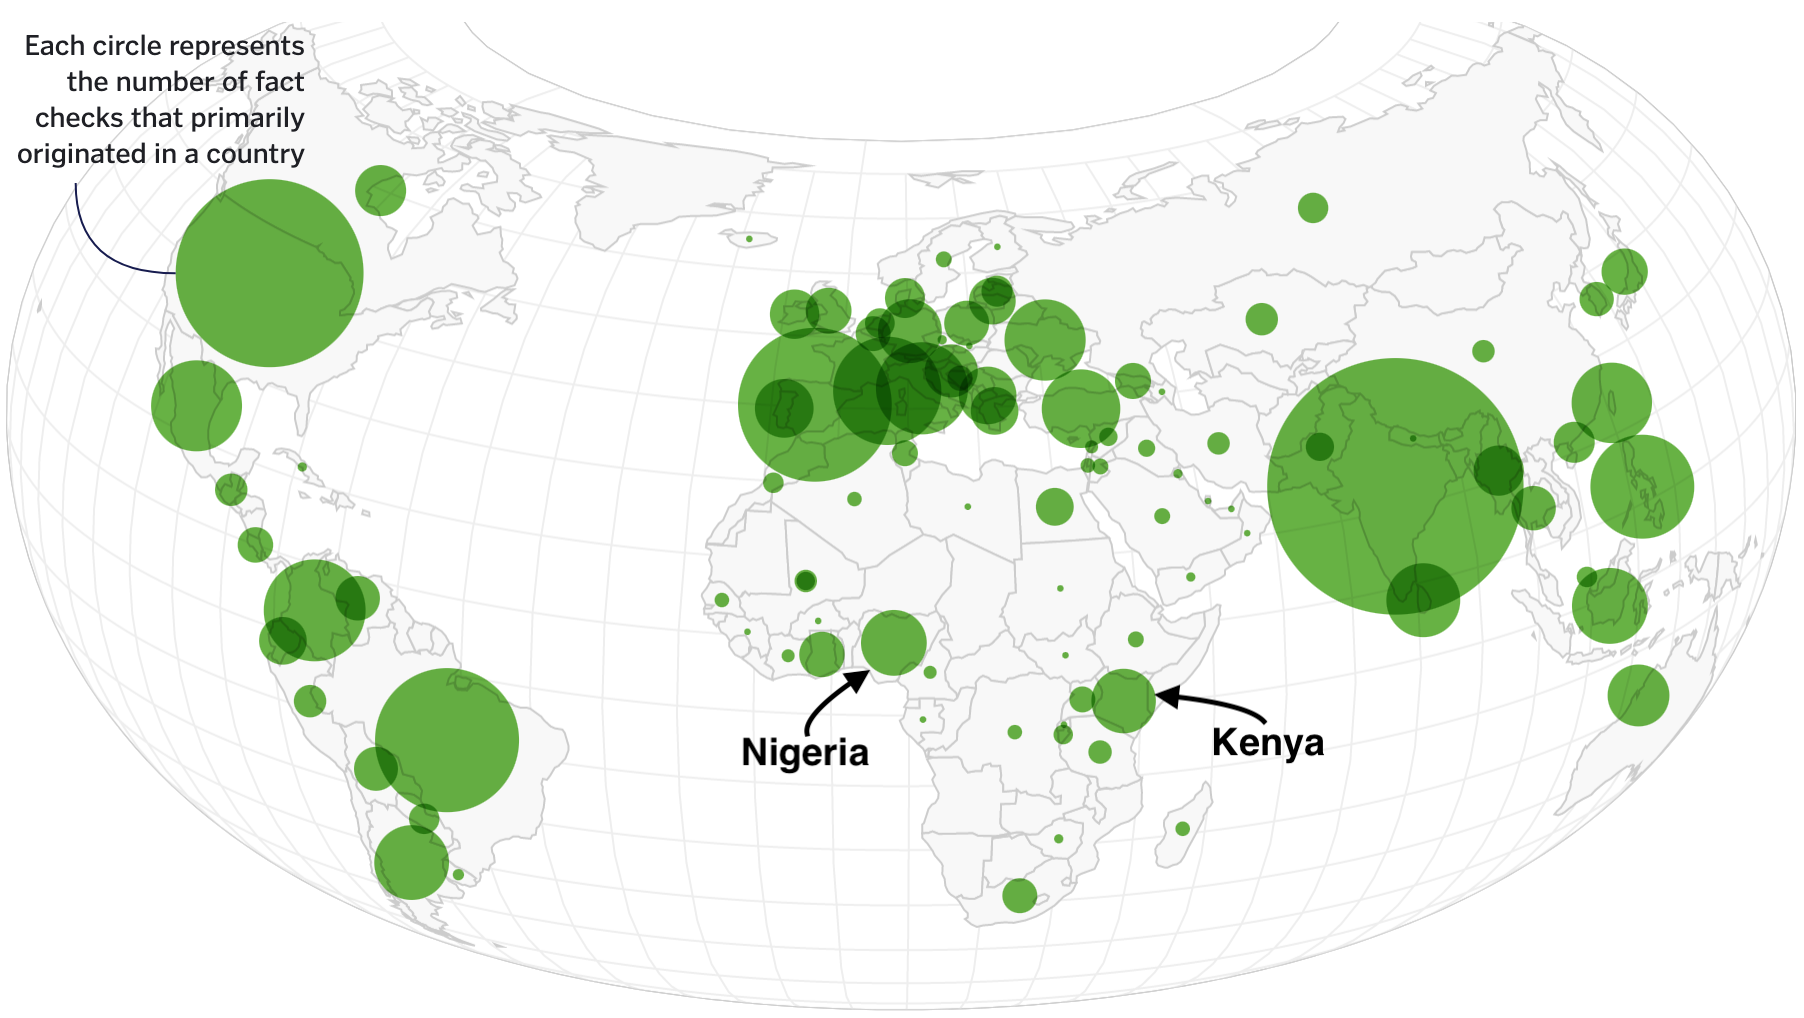
\includegraphics[width=.95\textwidth]{figures/poynter2.png}
\end{figure}

For this experiment, we focus on COVID-19 prevention and cure-related information because this comprises a large proportion of the overall coronavirus-related information that has been fact-checked by experts (see Figure \ref{fig:poynter_cures}) and also serves as some of the most dangerous misinformation. Some hoax cures, when adopted, can be deadly. Moreover, even if not adopted when claims about the existence of a cure circulate widely they may deter people from taking preventative measures. We acknowledge that interventions will likely need to be specific to the particular type of misinformation being targeted, whether political, health-related, etc. The focus of this paper is on prevention and cure-related (mis)information that is immediately relevant for the ongoing pandemic. 
%\todo{Should this be moved to a new 3.3.2 Stimuli section?} - kept here and changed section heading


\begin{figure}[!htb]
\centering
\caption{Map illustrating the volume of COVID-19 cure-related fact-checks in \url{poynter.org}'s global coronavirus database.}
\label{fig:poynter_cures}
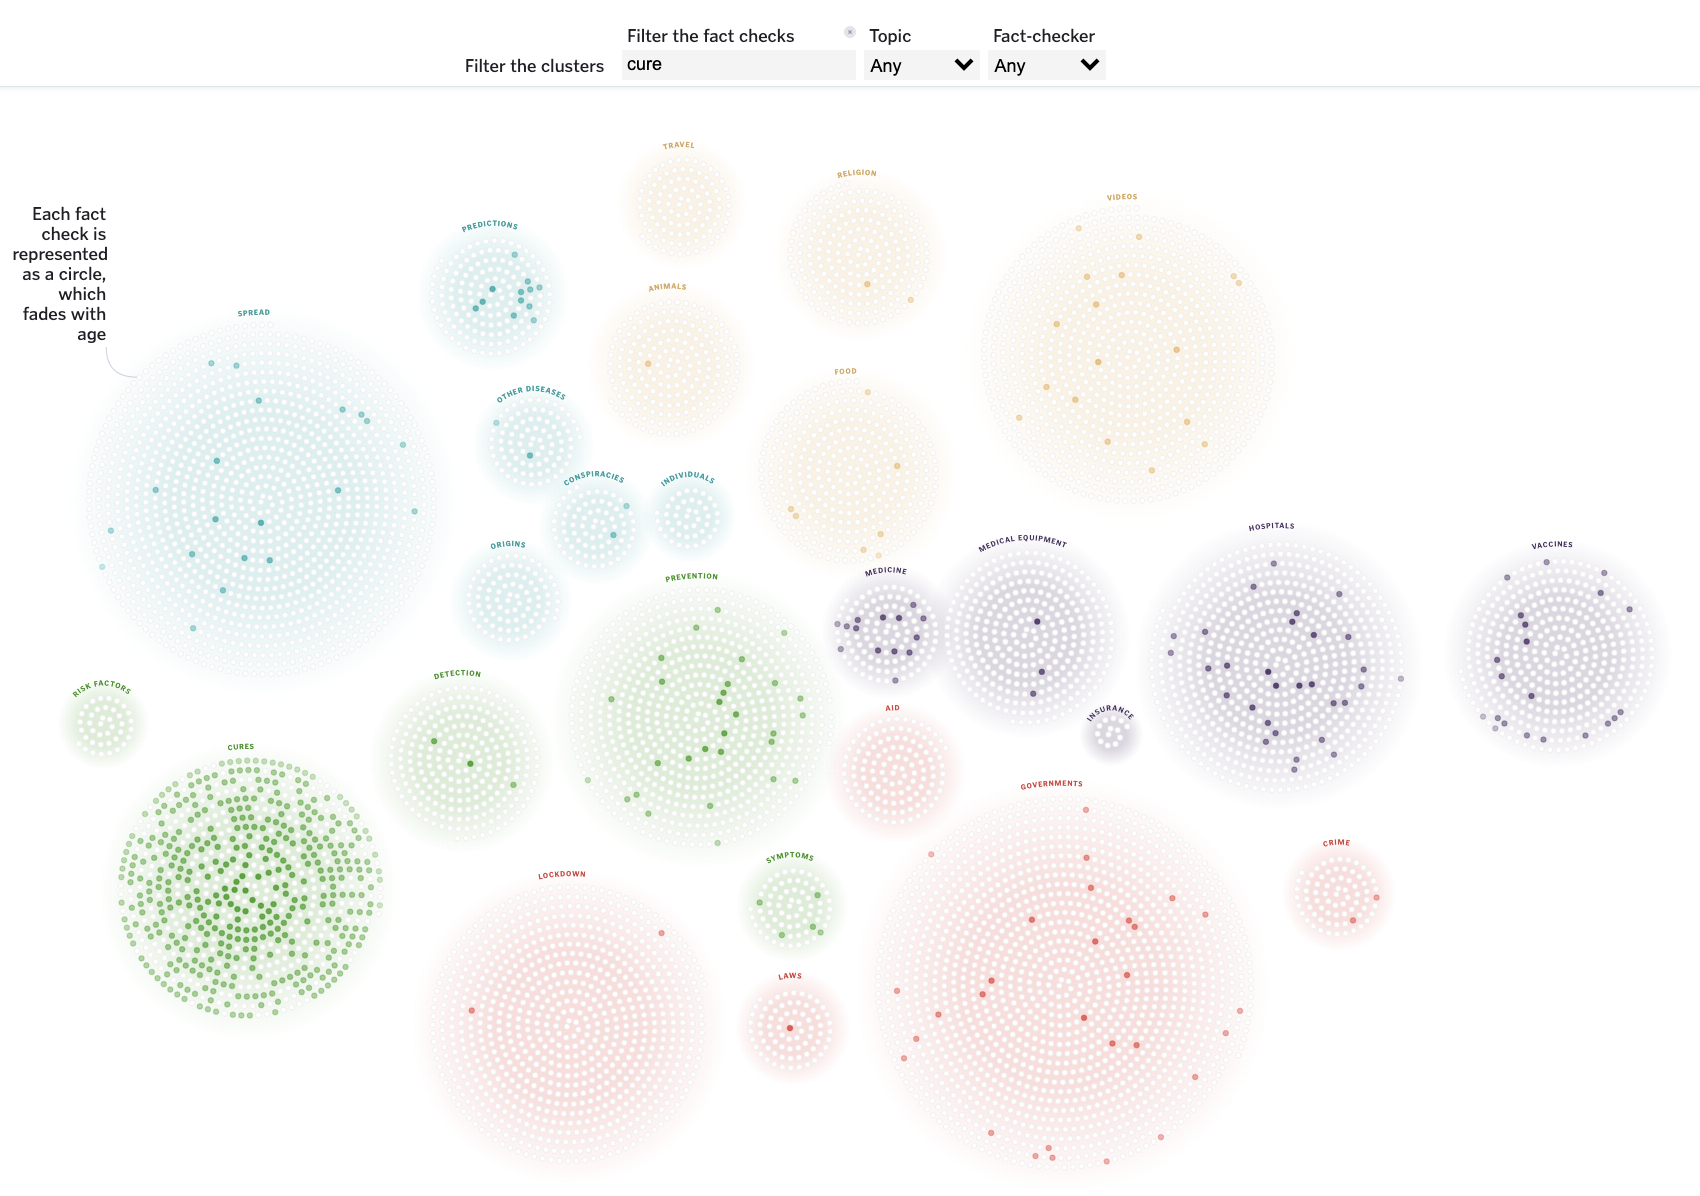
\includegraphics[width=.95\textwidth]{figures/poynter_cures.png} 
\end{figure}
% https://www.poynter.org/coronavirusfactsalliance/

To collect stimuli we adopted several criteria to search for both false and true pieces of information related to coronavirus prevention techniques and COVID-19 cures. First, we searched AFP, Poynter, and AfricaCheck websites for any of this type of misinformation that had been checked by these organizations that appeared online in Kenya and Nigeria since the start of the pandemic in early March 2020. Second, we collected WHO myth-buster infographics that directly countered the misinformation items we found. We also collected prevention messaging from the Nigeria Center for Disease Control, National Emergency Response Committee in Kenya, and the Ministry of Health in both countries, as these are the main government entities combating the spread of the disease in these countries and official sources of information. Our full set of stimuli for each country is provided in Appendix~\ref{appendix:stimuli}.\footnote{In addition to realism of the study, we use actual stimuli circulating online to avoid manufacturing our own ``cures'' and adding to the spread of online misinformation. Given that we use real media posts, some of our respondents may be familiar with these stories. To examine whether people were differentially discerning \citep{nyhan2020facts} or had different sharing preferences because they had previously seen these stimuli, we ask respondents at the end of the survey whether they had previously seen the stimuli.}

% People are more likely to endorse claims to which they have been exposed—at least absent effortful resistance (Gilbert, Tafarodi, and Malone 1993).







\FloatBarrier
\section{Experimental Setup}



\subsection{Sample recruitment}
We will recruit respondents in Kenya and Nigeria using Facebook advertisements targeted to users 18 years and older living in these countries.\footnote{Based on previous work it is clear that Facebook imputes location information for some of its users, which can be inaccurate \citep{Rosenzweig_2020}. We will also ask a location screening question to ensure our respondents live in our countries of interest.} %
To achieve balance on gender within our sample we create separate ads targeting men and women in both countries. Our target sample size is 1,500 respondents in each country for our pilot.\footnote{Assuming the maximum feasible variance under our response function, we calculate that this sample size will be sufficient to ensure that our estimate of the variance under the control condition will have an (asymmetric) 95\% confidence interval around the true variance with a width of 15\% of the true variance. This is relevant to ensure that our simulations discussed in Section~\ref{simulations} will be stable and appropriate to the setting.} Size of the full scale study will be determined following piloting, in procedures described in Section~\ref{simulations}. We anticipate that our sample will look similar to the overall Facebook population in these countries, which tends to be more male, more urban, and more educated than the overall population \citep{Rosenzweig_2020}. We will analyze how our sample compares to both the Facebook population and the general population in Kenya and Nigeria using Facebook's advertising API data and nationally representative Afrobarometer surveys conducted in both countries. 


Advertisements will appear within Facebook or Instagram, offering users with the opportunity to ``Take a 20 minute academic survey on Messenger - receive airtime.'' Incentives will be approximately 0.50-0.55 USD, accounting for transaction and messaging fees on the \href{https://africastalking.com/}{Africa's Talking} airtime distribution platform.%
\footnote{The recruitment advertisement is shown in Figure~\ref{fig:ad} in Appendix~\ref{appendix:recruitment}.} %
 When users click on the ``Send Message'' button on our advertisement, a Messenger conversation will open with our Facebook page, starting a conversation with a chatbot programmed to implement the survey.%
 \footnote{See Figure \ref{fig:chatbot} in Appendix~\ref{appendix:recruitment}.} % 
 In contrast to sending users to an external survey platform such as Qualtrics, the benefit of the chatbot is that we keep users on the Facebook platform, with which they are likely more familiar, and maintain a realistic setting in which users might encounter online misinformation.  Respondents who complete the survey in the chatbot will receive compensation in the form of mobile phone airtime sent to their phone. %%MOW: confirm survey completion time--and update advertisement accordingly




\subsection{Treatment}
Drawing on the literature on experimental interventions to combat misinformation, we include several treatments designed to reduce the spread of misinformation online, which are targeted both at the respondent level and the headline level. This list of treatments also draws on real-world interventions that companies and platforms have instituted to combat misinformation. Treatments are presented in Table~\ref{tab:treatments}; further details are presented in Appendix~\ref{sec:treatments}. 

Respondent-level treatments and headline-level treatments are implemented as separate factors, each of which has an empty baseline level that is the control. So respondents may be assigned the pure control condition, one of the respondent-level treatments but no headline-level treatment, one of the headline-level treatments but no respondent-level treatment, or one of the respondent-level treatments \textit{and} one of the headline-level treatments. 


% interesting point to maybe incorporate: Facebook, 24% of false-rated content in our sample remains up without warning labels \citep{brennen2020types}
%\todo{Add justification for emotion suppression treatment, per 9/1 meeting? Provide minimal justification for \textit{all}?}
\begin{table}[H]
\begin{adjustbox}{max width = \textwidth}
\begin{tabular}{l|l|l}
\multicolumn{1}{l|}{\textbf{\begin{tabular}[c]{@{}c@{}}Shorthand\\ Name\end{tabular}}} & \multicolumn{1}{c|}{\textbf{\begin{tabular}[c]{@{}c@{}}Treatment\\ Level\end{tabular}}} & \textbf{Treatment}                                                                                                                                                                                                                                                                                                                                                                                              \\ \hline
1. Facebook tips                                                                                                           & Respondent                                                                                                   &  Facebook's ``Tips to Spot False News'' 
\\
2. AfricaCheck tips                                                                                                         & Respondent                                                                                                   &  \url{Africacheck.org}'s guide: \\ & & ``How to vet information during a pandemic''                                                                                                                                                                                                                                                                                                                             \\
3. Video training                                                                                     & Respondent                                                                                                   &  Videos \href{https://www.facebook.com/Vodcasts/videos/1322816708106278/}{1}, \href{https://www.facebook.com/BBCnewsafrica/videos/3104356182956064/}{2}, \href{https://www.facebook.com/BBCMediaActionNaija/videos/195932528440760/}{3}                                                                                                                                                                                                                                                                                                                                                                                   \\
4. Emotion suppression                                                                                                       & Respondent                                                                                                   & \begin{tabular}[t]{@{}l@{}}Prompt: ``As you view and read the headlines, if you have any \\feelings, please try your best not to let those feelings show.  \\Read all of the headlines carefully, but try to behave so that \\someone watching you would not know that you are feeling\\ anything at all” \citep{gross1998emerging}.\end{tabular}
\\
5. Pledge                                                                                 & Respondent                                                                                                   &  \begin{tabular}[t]{@{}l@{}} Prompt: Respondents will be asked if they want to keep their\\ family and friends safe from COVID-19, if they knew \\COVID-19 misinformation can be dangerous, and if they're\\ willing to take either a \textit{private} or \textit{public} pledge to help identify\\and call out COVID-19 misinformation online (see \ref{sec:pledge}).
\end{tabular}
\\
6. Accuracy nudge                                                                                 & Respondent                                                                                                   & Placebo headline: ``To the best of your knowledge, is this\\& &headline accurate?'' \citep{pennycook2020fighting, pennycook_epstein_mosleh_arechar_eckles_rand_2019}.
\\
7. Deliberation nudge                                                                                 & Respondent                                                                                                   & Placebo headline: ``In a few words, please say \textit{why} you would\\ & & like to share or why you would not like to share this headline.''\\ & & [open text response]
\\
%Context                                                                                                        & Headline                                                                                                     & \begin{tabular}[t]{@{}l@{}}Facebook context button; if you click the info button on an\\ article, a pop-up tells you a few facts about the source: \\ how long the Facebook page has been registered,\\ and has a flag if article is more than 90 days old\end{tabular}
%\\
%Flag                                                                                                           & Headline                                                                                                     &  ``Disputed" flag on the headline                                                                                                                                                                                                                                                                                                                                                     \\
8. Related articles                                                                                                       & Headline                                                                                                     & Facebook-style related stories: below story,\\ & & show one other story which corrects a false news story                                                                                                                                                                                                                                                                                             \\
9. Factcheck                                                                                                      & Headline                                                                                                     & Fact checking flag from third party\\ & & PesaCheck or AfricaCheck
 \\
10. More information                                                                                                      & Headline                                                                                                     & Provides a link to ``Get the facts about COVID-19''\\
11. Real information                                                                                                      & Headline                                                                                                     & Provides a \textit{true} statement: ``According to the WHO,\\ & & there is currently \textbf{no proven} cure for COVID-19.
 \\
12. Control                                                                                                        & N/A                                                                                                          & Control condition                                                                                                                                                                                                                                                                                                                                                                                              
\end{tabular}
\end{adjustbox}
\caption{Description of interventions included in the experiment}
\label{tab:treatments}
\end{table}


Treatments 1, 2, 3, 8, 9 and 10 are derived from interventions currently being used by social media platforms including Facebook, Twitter, and WhatsApp. For instance, \citet{guessetal2020digital} find that reading Facebook's tips for spotting untrustworthy news improved participants' ability to discern false from true headlines in the US and India. Treatment 11 (real information) is a similar headline-level treatment that \textit{could be} adopted by industry partners. Rather than flags or warnings about \textit{mis}information, we test whether providing a simple true statement reduces sharing of false information. Existing research suggests that providing true information can sometimes influence individuals' attitudes and behaviors \citep{gilens2001political}. %depending on what video treatment used could also go here
Treatments 4, 6, and 7 are taken from previous academic studies. The accuracy nudge treatment (6) was specifically found to be effective at reducing the sharing of COVID-19 misinformation among respondents in the US. Our deliberation nudge treatment (7) was adapted from \citet{bago2020fake} that found asking respondents to deliberate to be effective at improving discernment of online political information. Emotions have been suspected to influence susceptibility to misinformation \citep{martel2019reliance}, our test evaluates one canonical method of emotion suppression as a way to reduce the influence of misinformation. The pledge treatment (5) was adapted from the types of treatments used by political campaigns to get subjects to pledge to vote or support a particular candidate \citep{costa2018walking}. %This kind of treatment has also been used in diverse cases, such as promoting abstinence among teens (CITE) and xxx. 
We vary whether the pledge is made in private (within the chatbot conversation) or in public (posted on the respondent's Facebook timeline) to test whether public pledges are more effective at influencing behavior than private ones \citep{cotterill2013impact}.\footnote{In the pilot we will A/B test specifics of the video training and the pledge treatments. We will evaluate the effectiveness of the different variations and then run whichever version proves more successful at reducing the sharing of false stimuli for the full-scale experiment.}



%\textbf{MORE on why these treatments:}
%1. Guess et al - forthcoming - who find that FB tips for spotting fake news improved discernment in the US + India (Nyhan 2020, p.231)
%2. nigeria data suggest correlation between feeling sad and afraid with improved discernment between true/false stimuli and associated with greater sharing intentions of true (more than false) stimuli -- but other work from US (non-covid) suggests emotion regulation can help improve discernment -- 
% Feeling happy and experiencing cognitive ease provides people with a signal that everything is going well—and it leads them to rely on their intuition. Feeling sad or experiencing metacognitive difficulty, in contrast, signals that everything is not going well. This can trigger the motivation to be more careful and deliberate (Alter, Oppenheimer, Epley, & Eyre, 2007; Bless, Schwarz, & Wieland, 1996; Isen, Nygren, & Ashby, 1988, but see Meyer et al., 2015 and Thompson et al., 2013).


\subsection{Covariates}

Covariate measurement plays an important role in our contextual adaptive design. We assign treatment conditional on context, where the context is defined by the measured pre-treatment covariates. (Procedures for treatment assignment are detailed in Section ~\ref{adaptiveagent}; the full list of covariates and question wording is in Appendix~\ref{appendix:covariates}.)
The motivation for this \textit{contextual} adaptive experiment comes from the widely shared belief by misinformation scholars that \textit{context matters.} More specifically, scholars note that ``\dots not all misinformation is created equal, nor are all individuals equally susceptible to its influence'' \citep{wittenberg2020misinformation}. In addition to heterogeneity in individual susceptibility to misinformation, ``responses to corrections are likely heterogeneous'' \citep{swire2020searching}. Hence, we expect to observe heterogeneity in response to the treatments described in the previous section and explicitly incorporate this into our experimental design by pre-specifying the covariates that we anticipate to moderate response.

Despite the fact that many prominent scholars emphasize the importance of context and heterogeneity among individuals, misinformation research generally relegates heterogeneous response to secondary analyses. Moreover, the existing misinformation literature centered around studies conducted with respondents in North America and Europe, most often focuses on political ideology \citep{pennycook_epstein_mosleh_arechar_eckles_rand_2019}, cognition or inclination to deliberate \citep{bago2020fake}, and media literacy \citep{guessetal2020digital}. Our study expands this focus to explore heterogeneity with respect to additional respondent covariates. Outside of contexts where partisanship is a salient identity and lens through which individuals interpret news and information, what are the likely sources of heterogeneity in individuals' receptivity to interventions to combat the spread of misinformation?

In addition to the demographic covariates commonly used in social science research, we also include specific questions regarding knoweldge of and concern about COVID-19, an index of scientific views, beliefs about government efficacy in the current coronavirus pandemic, religious behaviors and beliefs, locus of control, and digital literacy. These variables capture what other researchers have suggested are primary sources of heterogeneity in responses to misinformation: age, analytical thinking (captured in our scientific beliefs index), and need for closure (captured in our concern regarding COVID-19 concern measurement and the beliefs about government efficacy measurement) \citep{wittenberg2020misinformation}. However, our primary objective is to learn an optimal policy conditional on covariates, and not to determine \textit{which} covariates matter, and by how much. %For this reason, we refrain from formalizing hypotheses regarding treatment effect heterogeneity.

% for paper - add here lazer et al study on misinfo in US


%\textcolor{red}{EDITING...Psychological need for control + uncertainty of pandemic → superstitious beliefs / magical thinking
%Locus of control is defined as ``a generalized attitude, belief, or expectancy regarding the nature of the causal relationship between one's own behavior and its consequences'' (Rotter, 1966).
% An individual with an internal locus of control will ``attribute outcomes to their own actions'' while an individual with an external locus of control will attribute it ``to circumstances beyond their control'' (Rotter, 1966).
%Understand differences in effort/motivation
%More internal locus of control associated with higher education/income
%Health outcomes (cite psych paper)
%}

% Several of our treatments also target these features, such as analytic thinking (the deliberation and emotion suppression treatments).  



% LR: I removed based on our slack convo -- and idea to cite the issue where these specific hypotheses are stated
%\textbf{Predictions about covariates/heterogeneity:}\todo{@Molly do you think we should include this kind of thing here?}\todo{@Leah, I would if anything put a few of these in a paragraph form, and say, "However, our objective is to learn an optimal policy conditional on covariates, and not to determine which covariates matter, and by how much. For this reason, we refrain from formalizing hypotheses regarding treatment effect heterogeneity." What do you think?}
%\textcolor{red}{
%\begin{enumerate}
%\item At a high level, we expect to see results such as individuals with low digital media literacy will be most affected by the respondent-level false news video training combined with the fact-check headline treatment. Younger respondents who have a high level of concern about COVID-19 will be most affected by the pledge treatment combined with the related articles or fact-check headline treatments.
%\item Individuals who are more literate with respect to digital media will be most affected by the headline-level treatments. We also expect more educated and less religious individuals to be more influenced by these treatments.
%\item More educated and less religious individuals will be less influenced by our accuracy nudge or deliberation nudge treatments.
%\item Emotion suppression and accuracy nudge treatments will be more effective for low CRT and older respondents.
%\item Contrary to existing research based in the US, we do not expect partisanship to interact with our treatments.
%\item Sides 2016 + Gilens 2001 (information treatment more effective on high knowledge ppl)
%\item we expect that religiosity and religious beliefs - as well as locus of control - to matter...
%\item in US social distancing measures adopted at higher rates in areas with more climate change believers %https://www.researchgate.net/profile/David_Van_Dijcke/publication/341001499_Belief_in_Science_Influences_Physical_Distancing_in_Response_to_COVID-19_Lockdown_Policies/links/5ea96a1e92851cb267633a3d/Belief-in-Science-Influences-Physical-Distancing-in-Response-to-COVID-19-Lockdown-Policies.pdf
%\end{enumerate}
%}

% education tells us to give ppl a certain kind of treatment
% correlation of covariates
% pick 2 policies - 2 treatments or 1 status quo - standard HTE analysis for binary analysis. 
% ** do ridge regression for factorial model <-- hypotheses. commit to reporting output from interaction ridge model + hierarchical regularization w/covariates. --> averages of diff factors.


% - include more covariates in the pilot and then subset for actual survey
%	- include a couple different measures of covariates



\subsection{Outcomes and Response Function}\label{response}

We are primarily interested in decreasing sharing of harmful false information about COVID-19 cures and treatments, however, we would simultaneously wish to constrain negative impacts on sharing of useful information about transmission and best practices from verified sources. Specifically, we are interested in three outcomes: (1) Self-reported intention to share a given story, (2) Actual behavior with respect to sharing that story\footnote{Although this is only measured for the \textit{true} headlines as respondents are not asked to share the falsehoods.}, (3) Willingness to share tips and information about misinformation more generally. For the primary response function below, we conduct policy learning and evaluation as discussed throughout Section~\ref{analysis}. For secondary outcomes, (excluding aggregated tallies discussed below), only analysis for main effects of factor levels will be conducted as described in Section~\ref{main}.  

\subsubsection{Primary Response Function}%\todo{SA: the description in 3.4.1 is hard to read.  I think a diagram would make it much easier to follow.}

We measure interest in sharing information through two questions:
\begin{itemize}
\item Would you like to share this post on your timeline? 
\item Would you like to send this post to a friend on Messenger?
\end{itemize}


By using a pre-test / post-test design  \citep{davidian2005semiparametric} %https://declaredesign.org/library/articles/pretest_posttest.html
and an index of repeated measures \citep{broockman2017design}, we aim to improve the efficiency of our effect estimation. 

\documentclass[border=10pt]{standalone}
\usepackage{tikz}
\usetikzlibrary{arrows.meta}
\tikzset{%
  >={Latex[width=2mm,length=2mm]},
  % Specifications for style of nodes:
            base/.style = {rectangle, rounded corners, draw=black,
                           minimum width=4cm, minimum height=1cm,
                           text centered, font=\sffamily},
  activityStarts/.style = {base, fill=blue!30},
       startstop/.style = {base, fill=red!30},
    activityRuns/.style = {base, fill=green!20},
         process/.style = {base, minimum width=2.5cm, fill=orange!15},
                          % font=\ttfamily},
}
\begin{document}    
% Drawing part, node distance is 1.5 cm and every node
% is prefilled with white background

\begin{tikzpicture}[node distance=1.5cm,
    every node/.style={fill=white, font=\sffamily}, align=center]
  % Specification of nodes (position, etc.)
 \node (pretreat)             [activityStarts]              {Pre-Treatment Stimuli \\ \small{[Random: 2 true/2 false]}};
%  \node (onCreateBlock)     [process, below of=start]          {onCreate()};
%  \node (onStartBlock)      [process, below of=onCreateBlock]   {onStart()};
%  \node (onResumeBlock)     [process, below of=onStartBlock]   {onResume()};
  \node (distract)      [process, below of=pretreat, yshift=-.5in]
                                                      {Distraction Module};
  \node (treat)      [activityRuns, below of=distract]
                                                      {Treatment};
  \node (posttreat)      [activityStarts, below of=treat]
                                                      {Post-Treatment Stimuli \\ \small{[Random: 2 true/2 false]}};                                                      
%  \node (onPauseBlock)      [process, below of=activityRuns, yshift=-1cm]
%                                                                {onPause()};
%  \node (onStopBlock)       [process, below of=onPauseBlock, yshift=-1cm]
%                                                                 {onStop()};
%  \node (onDestroyBlock)    [process, below of=onStopBlock, yshift=-1cm] 
%                                                              {onDestroy()};
%  \node (onRestartBlock)    [process, right of=onStartBlock, xshift=4cm]
%                                                              {onRestart()};
%  \node (ActivityEnds)      [startstop, left of=activityRuns, xshift=-4cm]
%                                                        {Process is killed};
%  \node (ActivityDestroyed) [startstop, below of=onDestroyBlock]
%                                                    {Activity is shut down};     
 
 
  % Specification of lines between nodes specified above
  % with aditional nodes for description 
%  \draw[->]             (pretreat) -- node[text width=3in]
%                                   {4 random stimuli (2 true/2 false)}(treat);
     \draw[->]             (pretreat) -- node[text width=4in]
                                   {1. Would you like to share this post on your timeline?\\2. Would you like to send this post to a friend?}(distract);
     \draw[->]             (distract) -- (treat);    
     \draw[->]             (treat) -- (posttreat);                                 
%   \draw[->]             (treat) -- node[text width=3in]
%                                   {4 random stimuli (2 true/2 false)}(posttreat);                                 
%  \draw[->]     (onCreateBlock) -- (onStartBlock);
%  \draw[->]      (onStartBlock) -- (onResumeBlock);
%  \draw[->]     (onResumeBlock) -- (activityRuns);
%  \draw[->]      (activityRuns) -- node[text width=4cm]
%                                   {Another activity comes in
%                                    front of the activity} (onPauseBlock);
%  \draw[->]      (onPauseBlock) -- node {The activity is no longer visible}
%                                   (onStopBlock);
%  \draw[->]       (onStopBlock) -- node {The activity is shut down by
%                                   user or system} (onDestroyBlock);
%  \draw[->]    (onRestartBlock) -- (onStartBlock);
%  \draw[->]       (onStopBlock) -| node[yshift=1.25cm, text width=3cm]
%                                   {The activity comes to the foreground}
%                                   (onRestartBlock);
%  \draw[->]    (onDestroyBlock) -- (ActivityDestroyed);
%  \draw[->]      (onPauseBlock) -| node(priorityXMemory)
%                                   {higher priority $\rightarrow$ more memory}
%                                   (ActivityEnds);
%  \draw           (onStopBlock) -| (priorityXMemory);
%  \draw[->]     (ActivityEnds)  |- node [yshift=-2cm, text width=3.1cm]
%                                    {User navigates back to the activity}
%                                    (onCreateBlock);
%  \draw[->] (onPauseBlock.east) -- ++(2.6,0) -- ++(0,2) -- ++(0,2) --                
%     node[xshift=1.2cm,yshift=-1.5cm, text width=2.5cm]
%     {The activity comes to the foreground}(onResumeBlock.east);
  \end{tikzpicture}
\end{document}

Prior to treatment, we show respondents four media posts from their country (two true and two false in random order) randomly sourced from our stimuli set. For each stimuli we ask the above self-reported sharing intention questions (see Figure \ref{survey_flow}). Respondents are then asked a series of questions about their media consumption, and are then randomly assigned treatment according to the experimental design. If assigned to one of the respondent-level treatments, they are administered the relevant treatment. They are then shown four additional stimuli (two true and two false), selected from the remaining stimuli that they were \textit{not} shown pre-treatment. If the respondent is assigned a headline-level treatment, this treatment is applied only to the misinformation stimuli, as flags and fact-checking labels are not generally applied to true information from verified sources. For each of the stimuli we again ask the same self-reported sharing intention questions. 


%\todo{SA: on the randomization of the pre-treatment exposures, we can reduce variance by pre-randomizing combinations of pre-treatment exposures and treatments to ensure balance; this is a form of stratification.  For example, we create a set of vectors of pre-treatment exposures and treatment assignments that have the desired proportions, and then randomly assign participants to a member of the set (without replacement) upon arrival.  As Guido and I discuss in our handbook chapter on experimental design, it is always better to plan an experiment to avoid balance problems than to adjust for them afterwards.}

We code response to the self-reported questions as one if the respondent affirms they want to share the post and zero otherwise. Let $M_i^a$ be the sum of respondent $i$'s pre-test responses to the \textit{misinformation} stimuli and let $T_i^a$ be the sum of respondent $i$'s pre-test responses to the \textit{true} informational stimuli. $M_i^b$ and $T_i^b$ are the respective post-treatment responses. Then $M_i^a, T_i^a, M_i^b, T_i^b \in {0,1,2, 3, 4}$. 
%\todo{SA: the superscripts look like exponents.  Either change to letters or use double subscript, e.g. $M_{2,i}$.} 

We control for strata of pre-test responses in our analyses, i.e., $S=\{(m^a, t^a)\in M^a \times T^a\}$. 
We formalize our response function in terms of post-test measures:
\[
Y_i = -M^b_i + 0.5 T^b_i.
\]
This response function is the metric that we optimize for in our adaptive algorithm described in Section~\ref{adaptiveagent}, and in our policy learning described in Section~\ref{analysis}. Because of random assignment, we expect to see no systematic differences in pre-test interest in sharing either true or untrue stimuli across treatment conditions, conditional on covariates. %For a given treatment condition, all else equal, if respondents share misinformation at lower rates post-test compared to control, this will result in a relatively higher response variable. If respondents share true information at lower rates post-test compared to control, this will result in a relatively lower response variable, but the relative impacts are only half as large as those for the misinformation stimuli. 




\subsubsection{Secondary Outcomes}
Additionally, we measure secondary behavioral outcomes which allows us to further investigate the extent to which treatments may suppress the sharing of \textit{true} information.

In order to obtain a behavioral measure of sharing, we collect the articles the respondent indicated they would like to share throughout the survey and at the end of the survey provide links to the \textit{true} information. For these true stimuli, we offer respondents the opportunity to actually share this information as a Facebook post, which has been created on our project Facebook page. We are able to measure whether respondents click on a button which opens a pop-up screen to share the post on Facebook, however, we cannot measure directly whether they then actually follow through to the second step and post the article on their own timeline. Consequently, we report only rates of clicking the initial share button. The response function here is measured as the percent of true stimuli that the respondent said they wanted to share during the survey for which they later click the button to share on Facebook. (We do not differentiate between stimuli presented pre- and post- treatment here, since the behavioral response measurement for all stimuli is all post-treatment.) To provide some insight into the extent to which respondents followed up on an intention to share, we report the \textit{aggregate} number of times the associated post for each stimuli was shared. %We \textit{could} actually create a separate post for each treatment combination, and measure sharing that way, but this seems like overkill for a secondary outcome in an already complicated project.

At this point we also debrief respondents, informing them about the headlines they were shown that are false. Instead of allowing respondents to share these headlines, we provide links to tips for spotting misinformation online and also offer them the opportunity to share these tips on their timeline or on Messenger; we measure intention to share these tips as click-through-rates and aggregate number of shares of tips by treatment condition as well. 


\subsubsection{Attrition} We will include in analysis all respondents for whom we have collected complete pre-test responses. As treatment is not revealed at this point, attrition should be independent of treatment assignment conditional on covariates. For respondents who attrit after collection of pre-test responses and before collection of post-test responses, the post-test interest in sharing response function will be coded as identical to the individual pre-test value; for behavioral sharing outcomes, we impute zeros for click-through-rates.\footnote{An alternative approach to analysis in a pre-test/post-test design, accounting for missing data, would be to follow \cite{davidian2005semiparametric}'s implementation of estimators developed by \cite{robins1994estimation}.}


\section{Hypotheses and Data Collection}



Our data is described by treatments $W_i \in \ww$\footnote{Our treatments are composed of two separate factors, but here we use $W$ to represent combined treatment conditions, i.e., the unique combination of one respondent-level and one headline-level treatment. Where we wish to explicitly differentiate, we use $W^R_i$ and $W^H_i$ for respondent- and headline-level treatments respectively. Each factor includes a baseline level absent intervention, and the cardinality $|\ww| = |\ww^H|\times |\ww^R|$.}; response,  $Y_i \in \RR$; and covariates, $X_i \in \xx$. 

The data is indexed by $i = 1, \dots, N$ where indexing represents the order in which respondents entered the experiment; this allows us to use $i$ to also represent relative chronological relationships in our sequential adaptive design. 

We use potential outcome notation, where $Y_i(w)$ represents the potential outcome for respondent $i$ under treatment $w$.%, and by experimental design,  we have strong ignorability of potential outcomes to treatment conditional on observed covariates. 


We would like to learn and evaluate an optimal contextual policy, under which we assign the most effective treatment conditional on covariates. Formally, a policy maps a set of covariates to a decision \citep{athey2017efficient}, %\todo{Update reference}
\begin{align}
  \pi: \xx \rightarrow \ww. 
  \label{eq:policy}
\end{align}
In our setting, we will learn this policy, $\hat \pi$, and evaluate its value. The value of a policy is defined as, 
\begin{align}
V(\pi) =  \E[Y(\pi(X_{i}))],
  \label{eq:policy_value}
\end{align}
where the expectation is taken over the distribution of $X$.\footnote{Here we will only consider deterministic policies, but for a random policy, the expectation will be taken over the joint distribution of the covariates with the policy. }

\subsection{Hypotheses}\label{hypotheses}

\subsubsection{Optimal contextual and non-contextual policies}\label{policiesbest}
Our hypotheses of interest relate the value of an estimated optimal contextual policy $\pi_{opt}$ to fixed policies $\pi_{W}$, where under each fixed policy we would assign all respondents the relevant treatment $w$. The control policy is the fixed policy $\pi_{w^{C}}$

Our primary hypothesis is that we are able to estimate from the data an optimal contextual policy that improves value over the control. 
  \begin{hypothesis}
  The best contextual policy that can be estimated from the data achieves higher value than the control treatment. \label{eq:optctr}
\begin{align}
  H_{0}: V(\pi_{opt}) = V(\pi_{w^{C}}) \qquad H_{a}:  V(\pi_{opt}) > V(\pi_{w^{C}})
\end{align}
\end{hypothesis}
This is the hypothesis that we aim to optimize power for. 

We would also like to learn how much we gain by exploiting heterogeneity in the data. As secondary hypotheses, we propose that the optimal policy that we are able to estimate from the data improves over the best uniform respondent and headline level treatments; we learn these best uniform policies from the data, and test these hypotheses separately. 
\setcounter{hypothesis}{2}
  \begin{subhyp}
  The best contextual policy that can be estimated from the data achieves higher value than the best uniform headline-level treatment, i.e., the fixed headline-level treatment with the highest associated value. 
  \label{eq:optheadline}
\begin{align}
  H_{0}: V(\pi_{opt}) = \max_{w^H} V(\pi_{w^H}) \qquad H_{a}:  V(\pi_{opt}) > \max_{w^H} V(\pi_{w^H})
\end{align}
\end{subhyp}

  \begin{subhyp}
 The best contextual policy that can be estimated from the data achieves higher value than the best uniform respondent-level treatment, i.e., the fixed respondent-level treatment with the highest associated value. 
\begin{align}
  H_{0}: V(\pi_{opt}) = \max_{w^R} V(\pi_{w^R}) \qquad H_{a}:  V(\pi_{opt}) > \max_{w^R} V(\pi_{w^R})
\end{align}
\end{subhyp}

We discuss how we \textit{learn} these policies in Section~\ref{adaptivelearning}. 
%We test two secondary hypotheses regarding treatment effect heterogeneity. The literature on how age interacts with response to misinformation is not settled; \cite{wittenberg2020misinformation} note the attention given to age as an important moderator, and the finding that age correlates with propensity to share misinformation \citep[e.g.,]{guess2019less}, but echo the finding by \cite{amazeen2019reinforcing} that older respondents may be more likely to share fact-checks. Consequently, we test a two-sided hypothesis:


\subsubsection{Heterogeneous response}\label{policieshte}

While our main goal is to learn the best contextual policy -- and to see how this policy influences different types of people -- we also care about the outcome (reducing the spread of COVID-19 misinformation) and understanding which types of people are nudged toward this outcome by particular treatments. Therefore, we plan to examine how a few select treatments interact with particular covariates of interest. We do this in two ways - first by testing hypotheses particularly useful for industry and second by testing hypotheses driven by theoretical motivations, as described below.

\textbf{Hypotheses to inform industry practice:}
We select the below treatments because these are currently, or were previously, used by social media companies including Facebook and Twitter. The below covariates were selected as those that social media companies directly collect or have access to, and therefore could more easily use for targeting interventions. For our covariates of interest we will divide these into two groups for any binary variables (i.e. indicator for male) and split on the median value for continuous variables to test two subgroups (i.e. age $\geq$ median and age $<$ median). 

\textbf{Treatments:}
\begin{itemize}
\item Facebook tips (respondent)
\item AfricaCheck tips (respondent)
\item Factcheck (headline)
\item More information (headline)
\item Related articles (headline)
\end{itemize}

\textbf{Covariates:}
\begin{itemize}
\item Age
\item Male
\item Education
\end{itemize}

We hypothesize that the three headline-level treatments listed above will perform better among more educated users, older people, and among women, compared to the less educated, younger and male respondents. We expect that the two respondent-level treatments will reduce sharing of misinformation more among less-educated respondents than those with more education. %\footnote{After collecting pilot data we will submit an updated preanalysis plan in which we will specify and formalize exactly how we plan to test these hypotheses.}

\textbf{Hypotheses to inform social science theory:} Previous studies have hypothesized and tested the role that deliberation plays in mitigating belief and sharing of online misinformation \citep{bago2020fake,pennycook2020fighting}. Drawing on these findings, we anticipate that our \textit{accuracy nudge} and \textit{deliberation nudge} respondent-level treatments may help shift respondents from system I, intuitive reactions, to system II, more deliberative thinking by nudging respondents to stop and think about the accuracy of the headline, in the former, and about \textit{why} they share posts, in the latter. We anticipate that these treatments will perform comparatively better among respondents who score low on our CRT measure by getting these intuitive thinkers to stop and reflect. Alternatively, these treatments could perform best among high CRT respondents if they are better able to engage with these treatments in the desired way. 


% pledge hypotheses
We expect the pledge respondent-level treatment to be more effective among people who more frequently post and interact with friends on Facebook, those who are more religious (i.e. those who attend religious services more frequently), and those with high CRT scores. Among respondents who are randomly assigned the \textit{public} pledge treatment, we anticipate this treatment to be more effective among respondents who engage on Facebook regularly (as measured by the number of times they posted in the past 7 days and their frequency of communication with friends on the platform during the same period). In other words, we expect that people who are more engaged on social media, and therefore likely have more meaningful connections on the platform, will face higher audience costs to pledging to fight misinformation and then sharing dubious posts and will therefore reduce their sharing of misinformation. We also hypothesize that more religious respondents and those with high CRT scores, compared to their counterparts, may have stronger motivations to remain consistent with their own behavior. Meaning if they have pledged to helps spot misinformation, they will be less inclined to share it -- at least compared to those who may care less about commitment and consistency with their own previous actions. We evaluate heterogeneity with respect to intention to treat, i.e., individuals who were assigned to the pledge treatment, irrespective of whether they actually took the pledge. However, we will also report rates at which respondents clicked the button to share the pledge across groups under comparison.






% we may want to include measure of social media use as pretreatment covar
%\item \textit{We expect the real-information headline-level treatment to be more effective among those with a weaker internal locus of control, compared to those with a greater internal locus of control.} We anticipate that perhaps those who believe they have no choice at all over how their life turns out, once told that there is no cure for COVID-19 will be less likely to share ``cures'' with friends. 


\textbf{Best respondent and headline-level treatments:} In addition to the above hypotheses related to treatment heterogeneity, we also plan to test heterogeneity with respect to the best performing respondent-level and headline-level treatments. To estimate these we again take the median as the splitting point of continuous covariates to create ``high'' and ``low'' categories: 

Specifically, we will test:
\begin{enumerate}
\item How locus of control and age interact with the best uniform respondent-level treatment. 
\item How CRT and education interact with the best uniform headline-level treatment. 
\end{enumerate}


\subsubsection{Baseline levels}\label{baseline_levels}
In addition to response heterogeneity, we also anticipate that certain types of people are simply more likely to share false information, compared to true information. In particular, we expect that baseline rates of sharing false posts (compared to true posts) will be higher among these subgroups:
\begin{itemize}
\item young
\item male
%\item high internal locus of control
\item less educated
\item low CRT
\item more religious
\end{itemize}

% include language about baselines --> treatment effects?


%
%  \begin{hypothesis}
%Age will moderate treatment effect of the factcheck headline treatment relative to the control. 
%  \label{eq:age}
%  \begin{align*}
%  H_{0}: \E[ V(\pi_{w_{FC}}) -V(\pi_{w^{C}})|Age \ge  \emph{median } Age] = \E[ V(\pi_{w_{FC}}) -V(\pi_{w^{C}})|Age <  \emph{median } Age] \\
%   H_{a}:  \E[ V(\pi_{w_{FC}}) -V(\pi_{w^{C}})|Age \ge  \emph{median } Age] \neq \E[ V(\pi_{w_{FC}}) -V(\pi_{w^{C}})|Age <  \emph{median } Age] \numberthis
%\end{align*}
%\end{hypothesis}
%We note that because we do \textit{not} optimize for power for this hypothesis in our design; if the fact-check headline does not perform particularly well for either subgroup, it may be assigned to very few respondents. In that case, we will not be well-powered to test this hypothesis, and failure to reject the null may largely speak to a design under-powered for this test than absence of this heterogeneity. 
%
%
%
%Additionally, we test whether religiosity, as measured by frequency of attendance of religious services, moderates response to the real information headline treatment. In the real information treatment, we explicitly state that there is \textit{no proven cure} for COVID-19. We hypothesize that religiosity will \textit{negatively} correlate with response to this treatment. 
% \begin{hypothesis}
%Religiosity will moderate treatment effect of the real information headline treatment relative to the control. 
%  \label{eq:age}
%  \begin{align*}
%  H_{0}: \E[ V(\pi_{w_{FC}}) -V(\pi_{w^{C}})|Age \ge  \emph{median } Religiosity] = \E[ V(\pi_{w_{FC}}) -V(\pi_{w^{C}})|Age <  \emph{median } Religiosity] \\
%   H_{a}:  \E[ V(\pi_{w_{FC}}) -V(\pi_{w^{C}})|Age \ge  \emph{median } Religiosity] \le \E[ V(\pi_{w_{FC}}) -V(\pi_{w^{C}})|Age <  \emph{median } Religiosity] \numberthis
%\end{align*}
%\end{hypothesis}
%Again, we note that the adaptive design constrains our power for this test in the case that the real information treatment is relatively ineffective for either subgroup, and we consequently have only small sample size for this treatment in those groups.  



\subsection{Adaptive data collection}\label{adaptiveagent}

To collect data with the objective of learning an optimal policy, we use a \textit{contextual bandit} algorithm, in which we sequentially update treatment assignment probabilities based on the observed history of treatment, response, and covariates. These types of algorithms navigate a tradeoff in \textit{exploration} of the response surface with \textit{exploitation} of those treatments which we have observed to be effective based on historical data. This allows us to continue to learn about treatment effect heterogeneity while improving outcomes over time \textit{within} the frame of the experiment. 

We will use a version of linear Thompson sampling \citep{agrawal2013thompson}. Under Thompson sampling \citep{thompson1933likelihood,thompson1935theory}, treatment is assigned according to the Bayesian posterior probability that each treatment is best. In linear Thompson sampling, this is generalized to allow the outcome to be a linear function of covariates. Under this approach, we denote contexts associated with counterfactual potential outcomes as $x_{[w]}$, where $x$ is the observed covariate vector, augmented by the treatment indicator(s) consistent with treatment $W =w$, and potentially treatment covariate interactions; let this vector be of length $d$ for all $w \in \ww$. 

We implement the linear model supposing that there is some unknown coefficient vector $\theta\in R^{d}$, such that the $\E[Y_i(w)|X_i = x] = x_{[w]}^\top \theta$. %\sim \mathcal{N}\left( x_{[w],i}^\top \theta, \nu\right)$.%\footnote{Note that the variance term here is different than the coefficient variance covariance matrix discussed below. We follow \cite{agrawal2013thompson} in setting $\nu$ as a term that accounts for the sample size, the dimensionality of the covariates, and the variance or bounding of the distribution; we note that in this implementation, it does not vary across treatment arms.} 
We assign treatment under the heuristic that the reward distribution is Gaussian, but, as \cite{agrawal2013thompson} note, we do not require the true reward distribution to be Gaussian for regret bounds to hold. 

%We assume the variance is constant within arms, i.e., $\hat\V[Y(w)|X = x] = \sigma^2_w$. The conditional reward function is modeled as being distributed,
%  \begin{align}
%    \mu_w(x) \sim \mathcal{N}({\mu}_w(x), {\sigma}_w^{2}(x)) \qquad %\text{for } s \in \{1, \cdots, S\} \text{ and treatment }w
%    \text{ for all treatments }w \in \ww
%  \end{align}


Our implementation roughly follows the balanced linear Thompson sampling algorithm described in \cite{dimakopoulou2017estimation, dimakopoulou2019balanced}, where the estimates $\hat\theta$ and $\hat\V[\hat\theta]$ are produced using weights to account for unequal assignment probabilities. We use a batched approach to updating, collecting data and then updating the treatment assignment model after each batch. We denote batches $\mathcal{I}_b$ for $b = 1, \dots, B$. Full details for the batch-wise linear Thompson sampling algorithm are provided in Algorithm~\ref{algg:bblts}; we present an overview below. 

\paragraph{Adaptive agent}\label{agent}

\begin{enumerate}
\item In the first batch, $b = 1$, we assign treatment uniformly at random. 

\item For equally sized batches $b = 2, \dots, B-1$:

\begin{enumerate}
   \item \label{step:fit} At the beginning of each batch, fit a ridge regression of the outcome regressed on observed treatment-augmented covariates; compute the minimum mean cross-validated error value of the penalization factor $\lambda^{CV}$ using the entire observed history of data. 
    This model with penalty factor $\lambda^{CV}$ produces our estimate of the coefficient vector $\hat \theta$ and variance, $\hat\V[\hat\theta]$.\footnote{
We use the below linear model for the length $d$ parameter vector $\theta$, 
\begin{align*}
\hat{Y}(W) | X & =
			\sum_{w^R} 1\{W^R = w^R\}\beta_{w^R}  +
			\sum_{w^H} 1\{W^H = w^H\}\beta_{w^H}  +\\ 
			& \sum_{w^R} \sum_{w^H}1\{W^R = w^R\} \times 1\{W^H =  w^H\}\beta_{w^{R,H}} +  \\
			& \sum_{\ell}  X_{[\ell]}{\beta}_{\ell} +\\
			& \sum_{w^R} \sum_{w^H}1\{W^R = w^R\} \times 1\{W^H =  w^H\}  X_{[\ell]} {\beta}_{w^{R,H}. \ell}.
			\numberthis
         \label{eq:linear_model_full}
\end{align*} 
The model is estimated using $L_{2}$ penalties for regularization, exclusive of the main treatment effects $\beta_{w^R}$ and $\beta_{w^R}$. 
%The model is estimated using $L_{2}$ penalties for regularization, exclusive of the main treatment effects $\beta_{w}$. 
Observations are weighted according to standard inverse probability weights using known assignment probabilities, following \cite{dimakopoulou2017estimation}, as in Equation~(\ref{eq:IPW}). %Stabilized inverse probability weights are discussed in Appendix~\ref{appendix:stabilized}. 

We assume covariates are mean-centered and scaled to have sample variance of one \citep{marquardt1980you}; in practice, this re-scaling occurs each time we fit the ridge regression. 
}

For each observation $i$ in batch $b$,
\begin{enumerate}
 \item Draw $M=1,000$ draws from $\tilde \theta ^{(m)} \sim \mathcal{N}\left(\hat \theta,\hat\V[\hat\theta]\right)$, and calculate the proportion of times each arm produced the maximum estimate under the counterfactual treatment augmented covariate profile  $x_{[w]i}$:
				\begin{align}
%    q_w(X_i) = \frac{1}{M} \sum_{m=1}^M 1\left\{ w = \argmax_w \{ x_i^\top \tilde \theta ^{(m)}_1, \dots, x_i^\top\tilde \theta_{|\ww|}^{(m)} \}  \right\}.
   q_w = \frac{1}{M} \sum_{m=1}^M 1\left\{ w = \underset{w}{\argmax} \{ x_{[1]i}^\top \tilde \theta ^{(m)}, \dots, x_{[|\ww|]i}^\top\tilde \theta^{(m)} \}  \right\}
				\end{align}
	These are the raw Thompson sampling probabilities. 	
\item In our algorithm, these probabilities are constrained by a pre-determined probability floor, $p$, and rescaled to sum to one, giving us $e_{1}, \dots, e_{|\ww|}$. 
%				\begin{align}
%     \tilde{q}_w & =\max\left\{q_w, p\right\} \\
%    e_w& = \frac{ \tilde{q}_w(X_i)}{\sum\limits_{w }\tilde{q}_w(X_i) }. 
%				\end{align}
%\item Denote the control condition $w^{C}$. 20\% of the sample is automatically allocated to the control condition--in addition to the scaled portion of the remaining sample that is assigned under Thompson sampling. The other probabilities are re-scaled accordingly. \todo{ Remove control over- augmented}
%      \begin{align}
%         e_{w_C}(X_i) & = 0.2 + 0.8\hat{q}_{w_C}(X_i) \\
%          e_{w}(X_i) & = 0.8\hat{q}_w(X_i)\ \ \forall w \in \ww \setminus \{w_C\}. 
%      \end{align}
\item Assign treatment  according to the calculated probabilities: \\
$w_i \sim \textrm{Multinom} \left( e_{1}, \dots, e_{|\ww|} \right)$
\end{enumerate}
\end{enumerate}

\item For the final batch,  $b = B$, learn policies and collect data for evaluation. 

At the beginning of the batch, 
\begin{enumerate}
%$ Point-wise optimal policy
%  \item Fit a point-wise optimal policy  by taking the maximum of predicted values for each possible context $x$ 
%    \begin{equation}
%     \hat{\pi}_{x} = \argmax_{ w } \hat{\mu}_{w}(x) . 
%    \end{equation} 
  \item Fit an optimal depth\textcolor{black}{-two} policy tree, and learn the best uniform headline-level policy and the best uniform respondent-level policy. Approaches to learning these policies are described in Section~\ref{analysis}, below. 
%    \begin{align*}
%      \hat{\pi}_{opt} = \arg\max_{\pi \in \Pi}
%      \sum_{i \in \bigcup\limits_{b=1}^{B-1} \mathcal{I}_{b} }
%      \langle \pi(X_{i}), \hat{\Gamma}_{i, \cdot} \rangle \\
%       \text{where } \Pi \text{ is the class of depth-\textcolor{black}{two} policy trees.}
%    \end{align*}
  \item For each observation $i$ in the final batch, assign treatment with equal probability to:\label{step:policies}
  \begin{itemize}
  \item the pure control, 
  \item the best uniform headline level policy, with no respondent-level treatment, 
  \item the best uniform respondent-level policy, with no headline-level treatment, and
  \item the best contextual policy conditional on $x_i$, as determined by the policy tree object. 
  \end{itemize}
\end{enumerate}
\end{enumerate}


\section{Analysis}\label{analysis}

To learn the best uniform and contextual policies, we must conduct a preliminary evaluation on the adaptively collected data. We then use the last batch for final evaluation and hypothesis testing. To account for unequal treatment assignment probability, we use doubly robust scores $\Gamma_{i,w}$, as in (\ref{eq:DR}), following \cite{robins1994estimation}'s augmented inverse-propensity weighted scores, 

      \begin{align*}
        \Gamma_{i,w} = \mu_{w}(X_{i}) + 1 \{W_i = w \} \xi_w(X_i)(Y_{i} - \mu_w(X_i)). \numberthis\label{eq:DR}\\
         \mu_{w}(x)  = \E[Y_i(w) | X_i = x]
    \end{align*}

We estimate $\hat\mu_{w}(X_{i})$, the conditional mean for each $w$ using generalized random forests, as implemented by the \texttt{grf} package in \texttt{R} \citep{Tibshirani:2020aa}. 
%following the approach described in Appendix~\ref{appendix:grf}. 
$\xi_w(X_i)$ is a weight to account for unequal treatment assignment probabilities. %; we may use inverse probability weights calculated from the actual probabilities assigned under the experimental design; in practice, we use the stabilized versions of these weights, as described in Appendix~\ref{appendix:stabilized}.  %Again, we can use the full covariate set, as described in Appendix~\ref{appendix:covariates}, including the pre-test response measures on the righthand side of the model.
%Our methods for analysis will differ depending on how the data is collected.
We use inverse probability weights, 
\begin{align*}
\xi^{IPW}_w(X_i) = \frac{ 1 }{e_{w}(X_i)} \label{eq:IPW} \numberthis\\
e_{w}(x) = \Pr[W_i = w|X_i = x].
\end{align*}
Here, we can directly plug in the respective treatment assignment probabilities from the experimental design for the $e_{w}(X_i)$. 
 

\subsection{Policy learning and evaluation on adaptively collected data}\label{adaptivelearning}%\todo{SA: the covariate distributions may be a little different between the last batch and the rest of the batches, just due to sampling variation; one might mention that if they are, we might re-weight the last batch so that the mean values of x’s are the same.  This is mainly an issue if the X’s are very important and the covariate space has high dimension.}
%For adaptively collected data, as in the simulations discussed in Section~\ref{simulations} and our eventual experiment, we conduct policy learning and evaluation as below:

\begin{enumerate}
%\subsection{Adaptively weighted doubly-robust estimation} %\todo{Add appropriate reference to LFO paper.}
%\label{appendix:DRlfo}
\item \textbf{Compute doubly robust scores}. For adaptively collected data, we use doubly robust scores as in (\ref{eq:DR}), but due to the dependent nature of the data, to avoid bias, we must ensure that we use only historical data in our estimates of the nuisance components. 

The weights $\xi^{IPW}_w(X_i)$ are by design only produced from historical data. To estimate conditional means $\hat \mu_w(X_i)$, for each batch $b$ in $b = 1, \dots, B-1$ and for each treatment $w$:
\begin{enumerate}
\item Fit a random forest estimator on the observations assigned $w$ in batches up to and including batch $b$. 
\item For observations assigned $w$ in batch $b$, calculate $\hat\mu_w(X_i)$ using out-of-bag predictions. 
\item For observation \textit{not} assigned $w$ in batch $b$, calculate $\hat\mu_w(X_i)$ using regression forest predictions from the fitted model in step a. 
\end{enumerate}

 Compute doubly robust scores $\hat{\Gamma}_{i,w}$ plugging the estimated nuisance components into (\ref{eq:DR}). 
\item \textbf{Learn policies}. We learn policies on the data collected up to batch $B-1$, by taking the average of scores over the relevant evaluation sets $\mathcal{I}$, where $\mathcal{I}_b$ represents the set of all observations within batch $b$.
\begin{enumerate}
\item For the optimal contextual policy, estimate an optimal depth-two policy tree. 
%We have already fitted and stored an optimal policy to conduct the (nearly) on-policy evaluation in the final batch $B$ of the adaptive experiment. 
    \begin{align*}
      \hat{\pi}_{opt} = \arg\max_{\pi \in \Pi}
      \sum_{i \in \bigcup\limits_{b=1}^{B-1} \mathcal{I}_{b} }
      \langle \pi(X_{i}), \hat{\Gamma}_{i, \cdot} \rangle \\
       \text{where } \Pi \text{ is the class of depth-\textcolor{black}{two} policy trees.}
    \end{align*}
    To ensure we learn an optimal policy that is contextual, if we learn a policy where in the policy tree object, all of the actions are equivalent across leaves (i.e., the policy is not contextual), we remove this fixed treatment and re-learn the tree policy on the remaining treatments; we repeat this until we learn a non-uniform policy. 
    %\todo{\texttt{policy\_tree} doesn't have min node size, as in grf; to-follow up on possible approaches for implementing this. }
    
  \item We conduct evaluation of fixed policies on the adaptively collected data. %We note that evaluation of the optimal policy is simplified, due to the on-policy evaluation in the final batch $B$:
      \begin{align}
          \hat{V}({\pi}_{w})  &:= \frac{1}{\bigg{\lvert} \bigcup\limits_{b=1}^{B-1} \mathcal{I}_{b} \bigg{\rvert}} \sum_{i \in \bigcup\limits_{b=1}^{B-1} \mathcal{I}_{b} } \hat{\Gamma}_{i,w}
        \end{align}  
   To learn the \textbf{best uniform headline-level policy}, we average over all treatment combinations that include a given headline treatment; effectively, this marginalizes over a balanced distribution of the respondent-level policies. 
      \begin{align}
                          \hat{V}({\pi}_{w_H})  &:= \frac{1}{\bigg{\lvert} \bigcup\limits_{b=1}^{B-1} \mathcal{I}_{b} \bigg{\rvert}} \sum_{i \in \bigcup\limits_{b=1}^{B-1} \mathcal{I}_{b} } \hat{\Gamma}_{i,w}, \ \ w \ni w_H \\
w_H^* & =  \argmax_{w_H} \  \hat{V}({\pi}_{w_H})
\intertext{ The procedure is equivalent for learning the \textbf{best uniform respondent-level policy.}}
          \hat{V}({\pi}_{w_R})  &:= \frac{1}{\bigg{\lvert} \bigcup\limits_{b=1}^{B-1} \mathcal{I}_{b} \bigg{\rvert}} \sum_{i \in \bigcup\limits_{b=1}^{B-1} \mathcal{I}_{b} } \hat{\Gamma}_{i,w}, \ \ w \ni w_R  \\
w_R^* & =  \argmax_{w_R} \  \hat{V}({\pi}_{w_R})
%                     \hat{V}(\hat{\pi}_{opt})  &:= \frac{1}{\big{\lvert}  \mathcal{I}_{B} \big{\rvert}} \sum_{i \in \mathcal{I}_{B} }
%                      Y_i  \\
%          \langle \hat{\pi}_{opt}(X_{t}), \hat{\Gamma}_{i, \cdot} \rangle
    \end{align}
%   \item To learn and evaluate the best fixed policy on a dataset, we again take the relevant approach described in Appendix~\ref{appendix:bestfixed}. 
\end{enumerate}
\item \textbf{Evaluate policies} We hold out the last batch of data for policy evaluation and hypothesis testing. This allows us to learn and evaluate policies on separate splits of the data, whereas we otherwise would be subject to bias in our policy evaluations from over-fitting. Additionally, when using adaptively collected data, we are not able to use standard cross-fitting techniques such as k-fold cross-validation, due to the temporal dependencies. 

The procedures for policy evaluation on data collected using simple random assignment, as in the pilot and simulations below, are described in Appendix~\ref{randomlearning}, but are parallel to the steps outlined above. %We again estimate nuisance components and compute doubly robust scores using only the last batch of the data. Note that in this last batch, we have just four policies of interest, as described in Step~\ref{step:policies} of the \hyperref[agent]{Adaptive Agent}. 
\end{enumerate}
The data collected from this study may be used for eventual application of a contextual implementation of the evaluation weighting method proposed in \cite{hadad2019confidence}, and advanced for contextual cases in \cite{zhan2020retrospective}. However, these methods will not be discussed in this pre-registration. 


\subsection{Hypothesis testing and other analysis}
To evaluate the hypotheses from Section~\ref{hypotheses}, we estimate means and standard errors of the (differences in) policies using the averages and standard deviations of the (differences in) relevant scores, and conduct frequentist hypothesis testing. 

For analysis regarding main effects and heterogeneity with respect to the best contextual and best uniform respondent- and headline-level policies, we use only the last batch of the data. %, calculating doubly robust scores as described in Appendix~\ref{randomlearning}. 

For analysis regarding main effects and heterogeneity with respect to pre-determined factor levels, we use the adaptively collected data up through batch $B-1$, calculating doubly robust scores as described in Section~\ref{adaptivelearning}. When considering a specific factor level, we marginalize over a balanced distribution of the other factor.\footnote{For example, if we are interested in average outcomes under the Pledge respondent-level treatment, we will take an average of scores for the Pledge treatment crossed with each of the headline-level treatments, including the baseline control.} %
We note that this is different from the realized distribution of the other factor, as the adaptive design is intentionally unbalanced--and distributions of the \textit{other} factors will vary from level to level. We calculate these quantities by averaging across the relevant scores, and taking the standard deviations of the averages. 

\subsubsection{Main effects of each factor level}\label{main}
For the primary response function as well as secondary outcomes discussed in Section~\ref{response}, we report average outcomes under each headline factor level and separately each respondent factor level, marginalizing over a balanced distribution of levels of the other factor.

\subsubsection{Treatment effect heterogeneity}
We report the policy tree object $\hat{\pi}_{opt}$ learned on the first $B-1$ batches of the data. In addition, we report the means and standard deviations of all covariates in each leaf in the evaluation split of the data. We note that absence of a given covariate in splitting does \textit{not} imply that the covariate is irrelevant for treatment effect heterogeneity, however, comparing the differences in covariate distributions across leaves can provide further insight into what may predict heterogeneous responses to treatment. 

To test hypotheses regarding specific heterogeneous response, as described in Section~\ref{policieshte}, we again average across the relevant scores, and compare estimates across the two groups. Given that testing these treatment-covariate combinations will result in a large number of unique tests, we will adjust for multiple hypothesis testing for response heterogeneity by reporting tests under both Bonferroni and Benjamini-Hochberg corrections.


%\subsection{Conditional means model}\label{ridge}
%For the primary response function as well as secondary outcomes discussed in Section~\ref{response}, we report coefficient estimates from  a factorial conditional means model, where we conduct variable selection for interaction terms, and then conduct inference on the selected model (similar to the covariate-selection approach proposed by \citealt{bloniarz2016lasso}).  We use the following formulation in the variable selection model:
% 
%\begin{align*}
%\hat{\mu}_w(X_{i}) & =
%			\sum_{w^R} 1\{W^R_i = w^R\}\hat\beta_{w^R}  +
%			\sum_{w^H} 1\{W^H_i = w^H\}\hat\beta_{w^H}  +\\ 
%			& \sum_{\ell}  X_{[\ell]i}\hat{\beta}_{\ell} +\\
%			& \sum_{w^R} \sum_{w^H}1\{W^R_i = w^R\} \times 1\{W^H_i =  w^H\}\hat\beta_{w^{R,H}}. %+  \\
%			& \sum_{w^R} \sum_{w^H}1\{W^R_i = w^R\} \times 1\{W^H_i =  w^H\}  X_{[\ell]i} \hat{\beta}_{w^{R,H}. \ell}.
%			\numberthis
%         \label{eq:linear_model_full}
%\end{align*} 
%
%\begin{align*}
%\hat{\mu}_w(X_{i}) & =
%			\sum_{w} 1\{W_i = w\}\hat\beta_{w}  +
%			\sum_{\ell}  X_{[\ell]i}\hat{\beta}_{\ell} +
%			\sum_{\ell} \sum_{w}1\{W_i =  w\}  X_{[\ell]i} \hat{\beta}_{w, \ell}.\numberthis
%         \label{eq:linear_model_full}
%\end{align*} 
%The variable selection model uses $L_{1}$ penalties for regularization, exclusive of the main treatment effects $\beta_{w^R}$ and $\beta_{w^H}$. The OLS model includes only main effects and interaction terms. The models are estimated on the data from batches up to $B-1$. Covariates are mean-centered and scaled to have sample variance of one \citep{marquardt1980you}. Observations are weighted by their inverse probability weights, following \cite{vanderweele2010marginal}. %; regularization is hierarchically constrained over two levels of penalties, so that the penalty on covariate coefficients, the $\hat{\beta}_{\ell}$ terms, is less than or equal to the penalty on interaction of treatments or interaction of treatment with covariates, the $\hat\beta_{w^{R,H}}$ and $\hat{\beta}_{w^{R,H}, \ell}$ terms.  


\section{Simulations and design hyperparameters}\label{simulations}

\textit{\textbf{Note:} This section provides an overview of our approach to making data-driven design decisions. We will update this pre-analysis plan \textit{after} collecting pilot data and running simulations, to document simulation results and our final design hyperparameters, prior to implementing the eventual adaptive experiments. }

To carry out implementation, the above description requires setting of several design hyperparameters, including total experiment size $N$, number of batches $B$,  size of first batch $|\mathcal{I}_1|$, size of last batch $|\mathcal{I}_B|$, and probability floor $p$. 

We set these hyperparameters by learning from our pilot data of 1,500 observations from each country. In the pilot data, treatment is assigned uniformly at random. We conduct the below simulations \textit{separately} for each country, meaning that we may end up with meaningfully different designs in the two countries. 

We then simulate data generating processes (DGPs) based on the pilot data, with varying heterogeneity. We create these DGPs by fitting a model to each dataset following (\ref{eq:linear_model_full}), but instead of learning and applying the cross-validated penalty factor $\lambda^{CV}$, we generate models with varying complexity by over- and under-fitting to the data, imposing different penalty factors. In ridge regression, larger penalties will be associated with more parsimonious models, and less heterogeneity. Smaller penalties will be associated with more complex models, and consequently more heterogeneity. This approach allows us to simulate heterogeneity that would plausibly exist in the true underlying populations. 

We refer to the heterogeneity ``delta'' as the difference between the value of the best contextual policy and the best fixed policy, divided by the standard deviation of response under the best fixed policy. A delta of 0.5 would indicate that the best contextual policy returns response that is in expectation one half standard deviation higher than response under the best fixed policy. We can create a DGP with no heterogeneity by setting an arbitrarily large penalty factor, shrinking all treatment $\times$ covariate interactions to (effectively) zero. 


\paragraph{Data generating processes} 
The below procedures are bootstrapped 1,000 times. 
\begin{enumerate}
%\item Define a vector of potential $\lambda$ values, \textcolor{red}{[TK, inclusive of zero]}. 
\item  Sample $S=1,500$ observations with replacement from the empirical distribution of covariates in the pilot data; store this as $X^{(1)}, \dots,X^{(S)}$. 
\item Estimate heterogeneity deltas under each element of the vector of penalty factors:
\begin{enumerate}
\item Fit the model (\ref{eq:linear_model_full}) to the pilot data under the relevant penalty factor $\lambda$ to generate a model of predicted response conditional on covariates $\hat{Y}(W) | X$ for each treatment $w$.
%\footnote{The model is estimated using $L_{2}$ penalties for regularization, exclusive of the main treatment effects $\beta_{w}$. 
%\begin{align*}
%\hat{\mu}_w(X_{i}) & =
%			\sum_{w} 1\{W_i = w\}\hat\beta_{w}  +
%			\sum_{\ell}  X_{[\ell]i}\hat{\beta}_{\ell} +
%			\sum_{\ell} \sum_{w}1\{W_i =  w\}  X_{[\ell]i} \hat{\beta}_{w, \ell}.\numberthis
%         \label{eq:linear_model_full}
%\end{align*} 
%}
  \item Calculate predictions $\hat{Y}(W) | X^{(s)}$ under the above fitted model conditional on covariates $X^{(1)}, \dots,X^{(S)}$ for each treatment $w$. 
  \item Store values for fixed policies for each $w$
      \begin{align}
          \hat{V}({\pi}_{w})  &:= \frac{1}{S} \sum_{s = 1}^S \hat{Y}(w) | X^{(s)}  
          \end{align}
  \item Fit a point-wise optimal policy on the resampled data by taking the maximum conditional mean for each individual context $X^{(s)}$. Store the value for the optimal policy:
    \begin{align}
      \hat{V}({\pi}_{opt})  &:= \frac{1}{S} \sum_{s = 1}^S \max_{ w } \hat{Y}(w) | X^{(s)}
          \end{align}
  \item Compute the heterogeneity delta as $\left({V}({\pi}_{opt})-{V}({\pi}_{w_{max}})\right)/\hat\sigma_{w_{max}}$, where $w_{max}$ is the true best arm under the relevant conditional means model over the empirical distribution of covariates, and $\hat\sigma_{w}$ is the standard deviation of the relevant response \textit{in the pilot data}. 
\end{enumerate}
\item Search over the vector of potential penalty factors to find:
\begin{enumerate}
\item The factor with an associated heterogeneity delta that is closest in absolute distance to 0.05. This will allow us to learn about the performance of our algorithm in a case with a small amount of heterogeneity. 
\item The largest penalty factor within one standard deviation of cross validated error from no penalization. 
\item The two penalties factors which minimize the absolute distance to 1/3 and 2/3 of the distance between 0.05 and the above near-largest heterogeneity delta, so that we have four equally spaced heterogeneity deltas. 
\end{enumerate}
\end{enumerate}

\paragraph{Simulations}
This then gives us four conditional mean models for \textit{each} bootstrap iteration. We then generate data from these models by sampling covariates from the empirical distribution from the pilot data and assigning potential outcomes as the conditional means from the given model + a noise term, where the noise term is based on the mean error between the fitted model and the pilot data, estimated separately for each treatment. 

We run a series of simulated experiments using synthesized data from each of the DGPs, randomly applying hyperparameters from Table~\ref{tab:design}. 


\paragraph{Hyperparameter choice}
Our objective in selecting design hyperparameters is to optimize power for Hypothesis~\ref{eq:optctr}, while minimizing the size of the experiment and the number of batches. From the simulations we should be able to learn about power conditional on each combination of design hyperparameters. Our decision rule is as follows:
\begin{enumerate}
\item Estimate average power for Hypothesis~\ref{eq:optctr} under each unique combination of design hyperparameters, averaging across DGPs. 
\item If there is one or fewer combinations of design hyperparameters with average power $\ge.85$, select the set of design hyperparameters which optimizes Hypothesis~\ref{eq:optctr}. To break ties, select the set with smallest experiment size, or, if of equal size, select with smallest number of batches. If experiment size and batch size are equal, select randomly. 
\item If there is more than one combination of design hyperparameters with average power $\ge.85$, constrain choices to only those sets with average power $\ge.8$. Then constrain choices to only those sets with the smallest experiment size, and then to the smallest number of batches. Among the remaining sets, optimize for power of Hypothesis~\ref{eq:optctr}. To break ties, select randomly. 
\end{enumerate}

\begin{table}[H]
\centering
\caption{Design hyperparameters} 
\label{tab:design}
\begin{tabular}{l | l}
\textbf{Hyperparameter} & \textbf{Choice set} \\ \hline
Adaptive experiment size ($N^A = \bigg{\lvert} \bigcup\limits_{b=1}^{B-1} \mathcal{I}_{b} \bigg{\rvert}$ )& [1500:3000 (steps of 500)] \\
Number of batches ($B$)& [10, 15, 20] \\
First batch size ($|\mathcal{I}_1|$) & $N^A \times$ [1/5, 1/4, 1/3] \\
Last batch size ($|\mathcal{I}_B|$) & **  \\
%Outcome model & [Ridge, Random Forest] \\
%Balancing weights & [Batch-wise IPW, ARB]\\
Probability floor (p)& [0.1, 0.15, 0.2]$\times 1/ |\ww|$ \\
$N$ & $=N^A + |\mathcal{I}_B| $\\
\hline
\end{tabular}
\end{table}
**Last batch size $|\mathcal{I}_B|$ is set at 2,500, to sufficiently power a one-sided test of Hypothesis~\ref{eq:optctr}, where the optimal contextual policy is .15 standard deviations greater than the control policy. 

\section{Simulations}
To ensure the robustness of our adaptive design, we consider performance of our algorithm under hypothetical data generating processes (DGPs). Here, we use a simplified version of the design, where we consider only unique treatment interventions, not factorial combinations. We assume that across the DGPs, there are three groups, and within each group, conditional on covariates, a different arm gives the highest reward. We then vary:
\begin{itemize}
\item \textbf{Relative size of the groups.} We allow the largest group to be 0.4, 0.6, and 0.8 share of the underlying population, with the two remaining groups approximately equally sized.
%\item \textbf{Number of predictive covariates.} We vary the number of covariates used to predict group membership, over 3, 5, and 10 covariates. 
\item \textbf{Heterogeneity in the data.} We vary the relative value of the best contextual policy to the best fixed policy to be 0.02, 0.14, or .2.\footnote{These quantities were selected by setting the value of the best contextual policy as 1.05, 1.5, or 1.95 times greater than that of the best fixed policy, but in general, we prefer to present heterogeneity in terms of increases in standard deviations to ensure that this quantity is not dependent on shifts in the mean of the response function.} 
\end{itemize}

We simulate effect sizes that are equivalent to 0.6 in the scale of our response function. This would be the effect if respondents decreased their propensity to share misinformation stimuli by .1, and increased their propensity to share true information stimuli by .1. This is the magnitude of the average effect for the \textit{most effective treatment arm} within each group as compared to the control condition. Consequently, this is also the average treatment effect for the best contextual policy relative to the control. The average treatment effect for the best fixed policy then changes with heterogeneity deltas and relative group sizes, but it is strictly less than 0.6. 

We selected this magnitude of effect for simulations based on the findings in \cite{pennycook2020fighting}, where their measured outcome is similarly sharing intentions. They find the difference in propensity to report sharing intentions between true and false stimuli expands from 0.050 to 0.142, or nearly .1. This is the average effect for a single fixed treatment condition; we hypothesize a somewhat greater widening for the \textit{oracle} contextual policy, where the oracle policy would be the true best policy based on the simulated DGP. That said, we do not expect to learn the oracle policy in practice, and in the simulations below, the value of the estimated policies fall short of this oracle policy. 

A brief overview of the design of DGPs implemented in these simulations is provided in Appendix~\ref{appendix:dgp}. The features of the underlying DGPs primarily inform the value of the policy that is learned. Because we ensure that the value of the best contextual policy and the control policy are fixed across simulations, as we increase heterogeneity, all else equal, we have to decrease the value of the best fixed policy in regions where there is disagreement between the best contextual and the best fixed policy. Consequently, while the oracle contextual policy has the same value across simulations, the learned contextual policy may be of lower value in settings where there is more heterogeneity. %Increasing number of predictive covariates also makes it harder for the algorithm to correctly learn group membership. 


\FloatBarrier
\subsection{Overall power}
These simulations provide justification for the choice of design hyperparameters described in Table~\ref{tab:design}. We see that in the settings below, the adaptive algorithm achieves higher power than the random design at all timepoints; this is due to learning a higher value policy in the learning stage of the experiment, and in the evaluation stage, allocating treatment only to the policies of interest. 

In the figures below, we marginalize over a balanced distribution of the choice of design hyperparameters; we then consider each hyperparameter in turn. Careful choice of design hyperparameters as described in Section~\ref{simulations} will help us to learn higher value policies, optimizing for power. Note that in the x-axis below, we consider the size of the sample used to \textit{evaluate} the policies.  

\begin{figure}[ht]
\centering
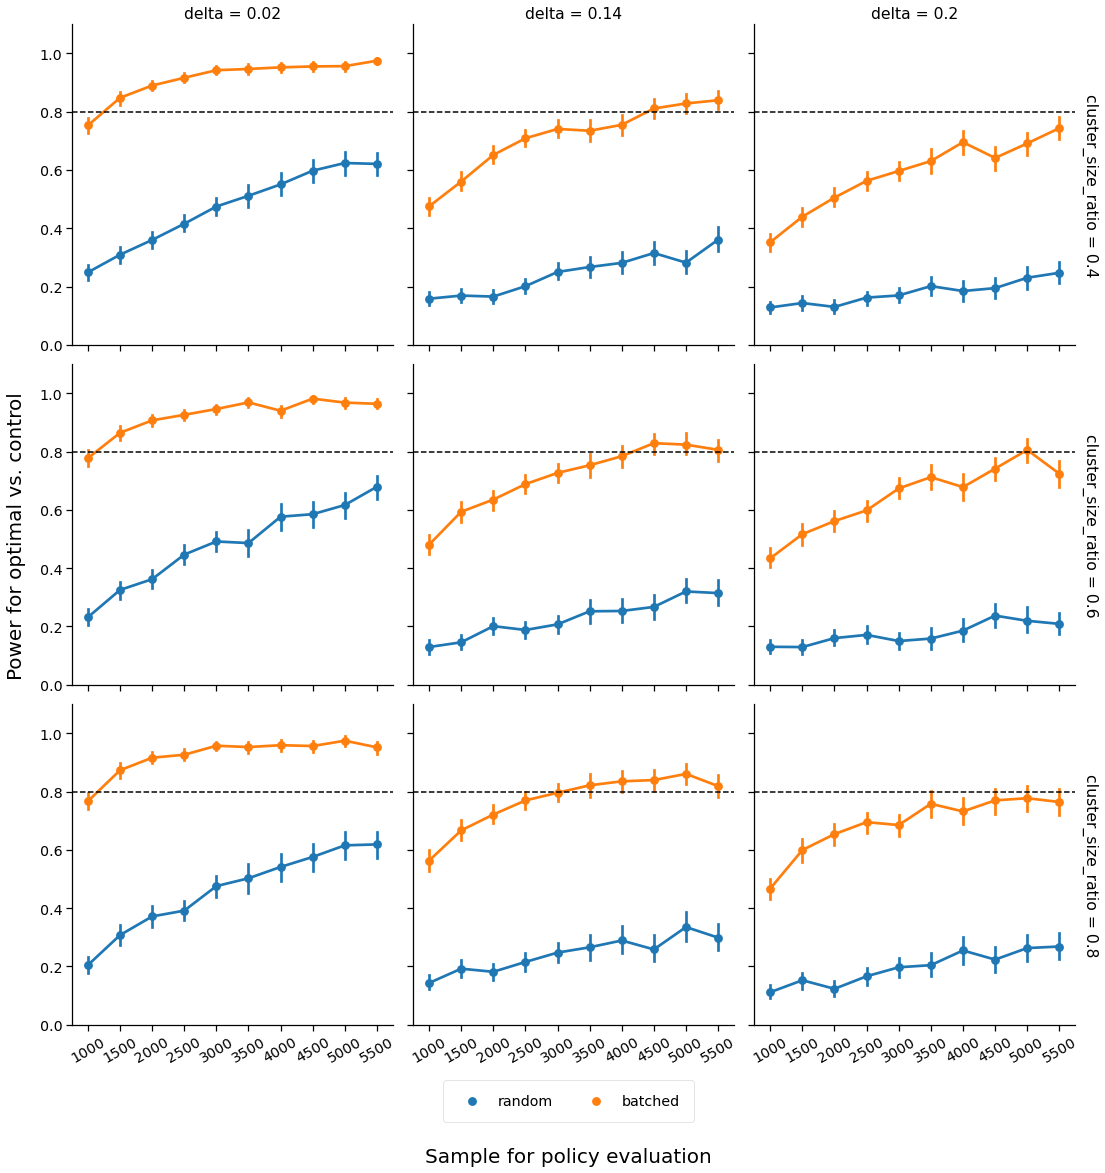
\includegraphics[width=.9\textwidth]{figures/power_against_control_policy_forest.png}
\caption{
%\textbf{Y-axis:} Power for the hypothesis that the estimated optimal policy is not equal to the control policy. 
%\textbf{X-axis:} Sample used for evaluation.\\
Rows represent the relative group size, where a cluster size of 0.4 indicates the group for whom the best fixed arm is best is 0.4 share of the underlying population, and the two remaining groups are each equally split.  Columns indicate heterogeneity delta. }
\label{fig:power_control}
\end{figure}\FloatBarrier

%
%\begin{figure}[ht]
%\centering
%\includegraphics[width=.9\textwidth]{figures/power_against_control_policy_forest_0.02.png}
%\caption{\textbf{Heterogeneity delta:} 0.02. \\
%\textbf{Y-axis:} Power for the hypothesis that the estimated optimal policy is not equal to the control policy. 
%\textbf{X-axis:} Sample used for evaluation.\\
%Columns represent the relative group size, where a cluster size of 0.4 indicates the group for whom the best fixed arm is best is 0.4 share of the underlying population, and the two remaining groups are each equally split. Rows indicate the number of covariates used to define group clusters. }
%\label{fig:power_control1.05}
%\end{figure}\FloatBarrier
%
%\begin{figure}[H]
%\centering
%\includegraphics[width=.9\textwidth]{figures/power_against_control_policy_forest_0.14.png}
%\caption{\textbf{Heterogeneity delta:} 0.14. \\
%\textbf{Y-axis:} Power for the hypothesis that the estimated optimal policy is not equal to the control policy. 
%\textbf{X-axis:} Sample used for evaluation.\\
%Power for the hypothesis that the estimated optimal policy is not equal to the control policy. Columns represent the relative group size, where a cluster size of 0.4 indicates the group for whom the best fixed arm is best is 0.4 share of the underlying population, and the two remaining groups are each equally split. Rows indicate the number of covariates used to define group clusters. }
%\label{fig:power_control1.5}
%\end{figure}
%
%\begin{figure}[H]
%\centering
%\includegraphics[width=.9\textwidth]{figures/power_against_control_policy_forest_0.2.png}
%\caption{\textbf{Heterogeneity delta:} 0.20. \\
%\textbf{Y-axis:} Power for the hypothesis that the estimated optimal policy is not equal to the control policy. 
%\textbf{X-axis:} Sample used for evaluation.\\
% Power for the hypothesis that the estimated optimal policy is not equal to the control policy. Columns represent the relative group size, where a cluster size of 0.4 indicates the group for whom the best fixed arm is best is 0.4 share of the underlying population, and the two remaining groups are each equally split. Rows indicate the number of covariates used to define group clusters. }
%\label{fig:power_control1.95}
%\end{figure}

\subsection{Varying parameters of the adaptive algorithm}
Aside from the last batch size, the design hyperparameters improve power by increasing the value of the estimated optimal policy. Note that in the x-axis in the following figures, we consider the size of the sample used to \textit{learn} the policies. 

We note that when there is very little heterogeneity in the data, we learn a better contextual policy using the randomly collected data. This may be because the adaptive algorithm exploits false leads, resulting in higher variance in the scores used for policy learning, without consequent benefit in more information on the best policies. 

In the below figures, we marginalize over the relative group size. % and the number of predictive covariates.  

\subsubsection{Varying probability floor}
We include probability floors in the adaptive algorithm. In the random algorithm, the floors are implicitly $ 1/ |\ww|$. Floors ensure that our weights are not too extreme when conducting estimation using inverse probability weights; floors that are too high may reduce the algorithm's ability to exploit promising arms.

\begin{figure}[H]
\centering
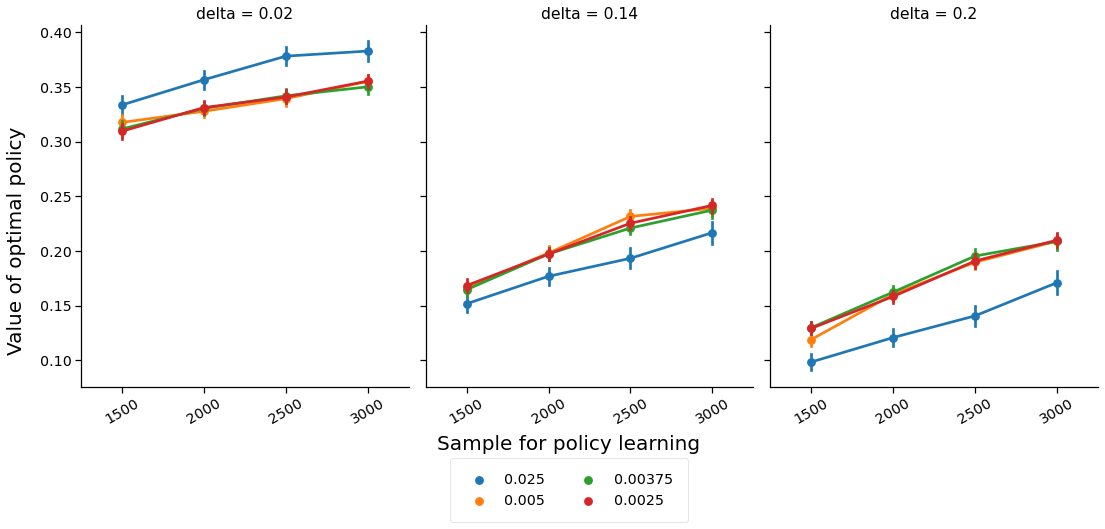
\includegraphics[width=\textwidth]{figures/value_diff_control_floor.png}
\caption{
%\textbf{Y-axis:} Value of the difference between the estimated optimal policy and the control policy. 
%\textbf{X-axis:} Sample used for policy learning.\\
 Hues represent the probability floors. A floor of 1/40 = 0.025 represents the random design. }
\label{fig:value_control_floor}
\end{figure}


\subsubsection{Varying first batch size}
In the adaptive algorithm, we explore randomly in the first batch. A larger first batch may reduce extreme probabilities, but inhibits our ability to exploit promising arms. The random algorithm has no set first batch. 

\begin{figure}[H]
\centering
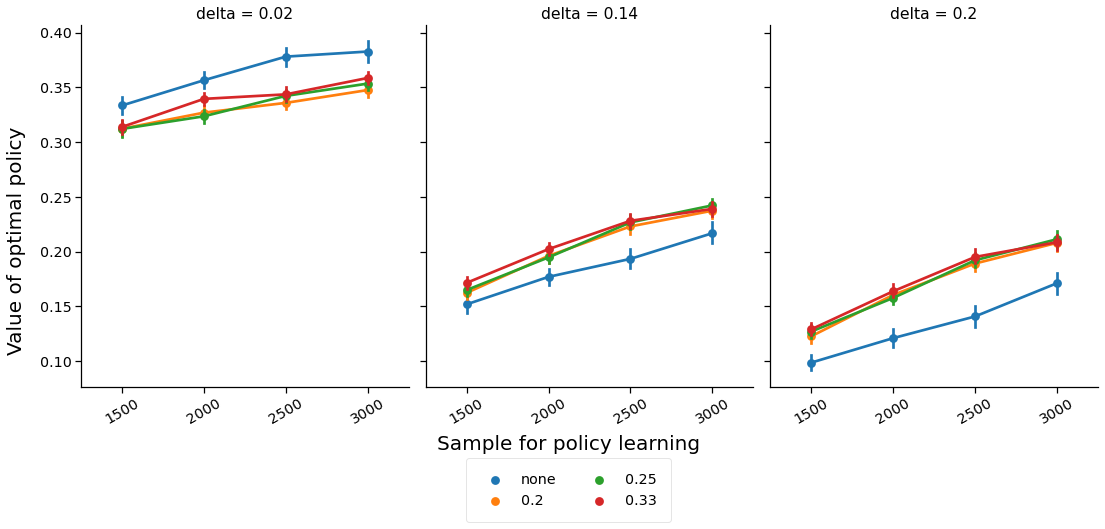
\includegraphics[width=\textwidth]{figures/value_diff_control_initial_batch_prop.png}
\caption{
%\textbf{Y-axis:} Value of the difference between the estimated optimal policy and the control policy. 
%\textbf{X-axis:} Sample used for policy learning.\\ 
Hues represent the proportion of the experiment assigned under random exploration in the first batch. }
\label{fig:value_control_initial_batch_prop}
\end{figure}

\subsubsection{Varying number of batches}
In the adaptive algorithm, we update the assignment algorithm in batches; more batches move us closer to a fully online algorithm. However, frequent updating may be computationally or logistically costly. The random algorithm never updates. 

\begin{figure}[H]
\centering
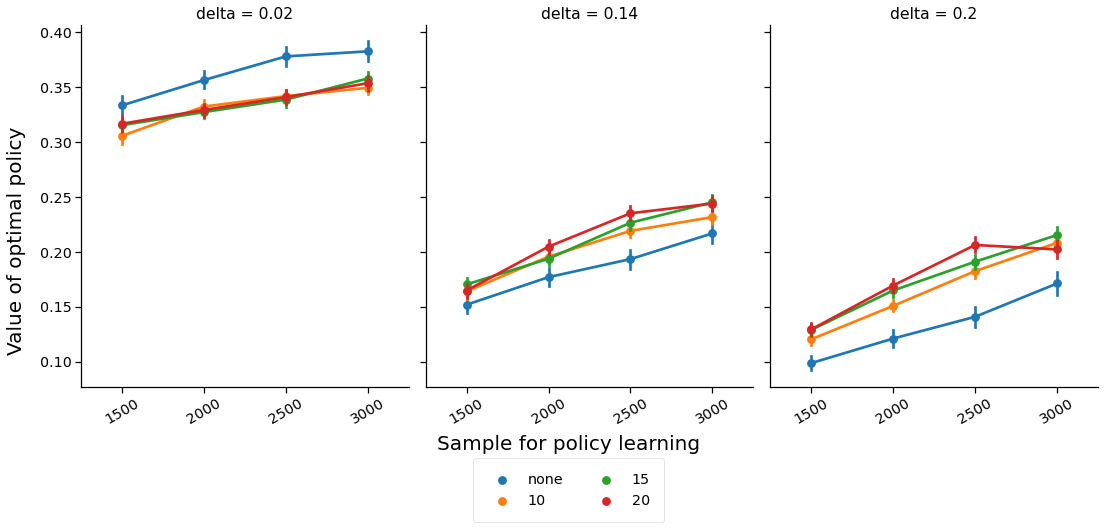
\includegraphics[width=\textwidth]{figures/value_diff_control_num_batches.png}
\caption{
% \textbf{Y-axis:} Value of the difference between the estimated optimal policy and the control policy. 
%\textbf{X-axis:} Sample used for policy learning.\\ 
Hues represent the number of batches between the first and last batch.}
\label{fig:value_control_batches}
\end{figure}


\clearpage
\bibliography{fb_misinfo_references}

\clearpage
\appendix

\section{Recruitment}\label{appendix:recruitment}
Respondents will be recruited through Facebook advertisements (Figure \ref{fig:ad}) that appear on their news feed, mobile application, and instagram. 

\begin{figure}[htb]
\centering
\caption{Advertisement as run in Facebook timeline.}
\label{fig:ad}
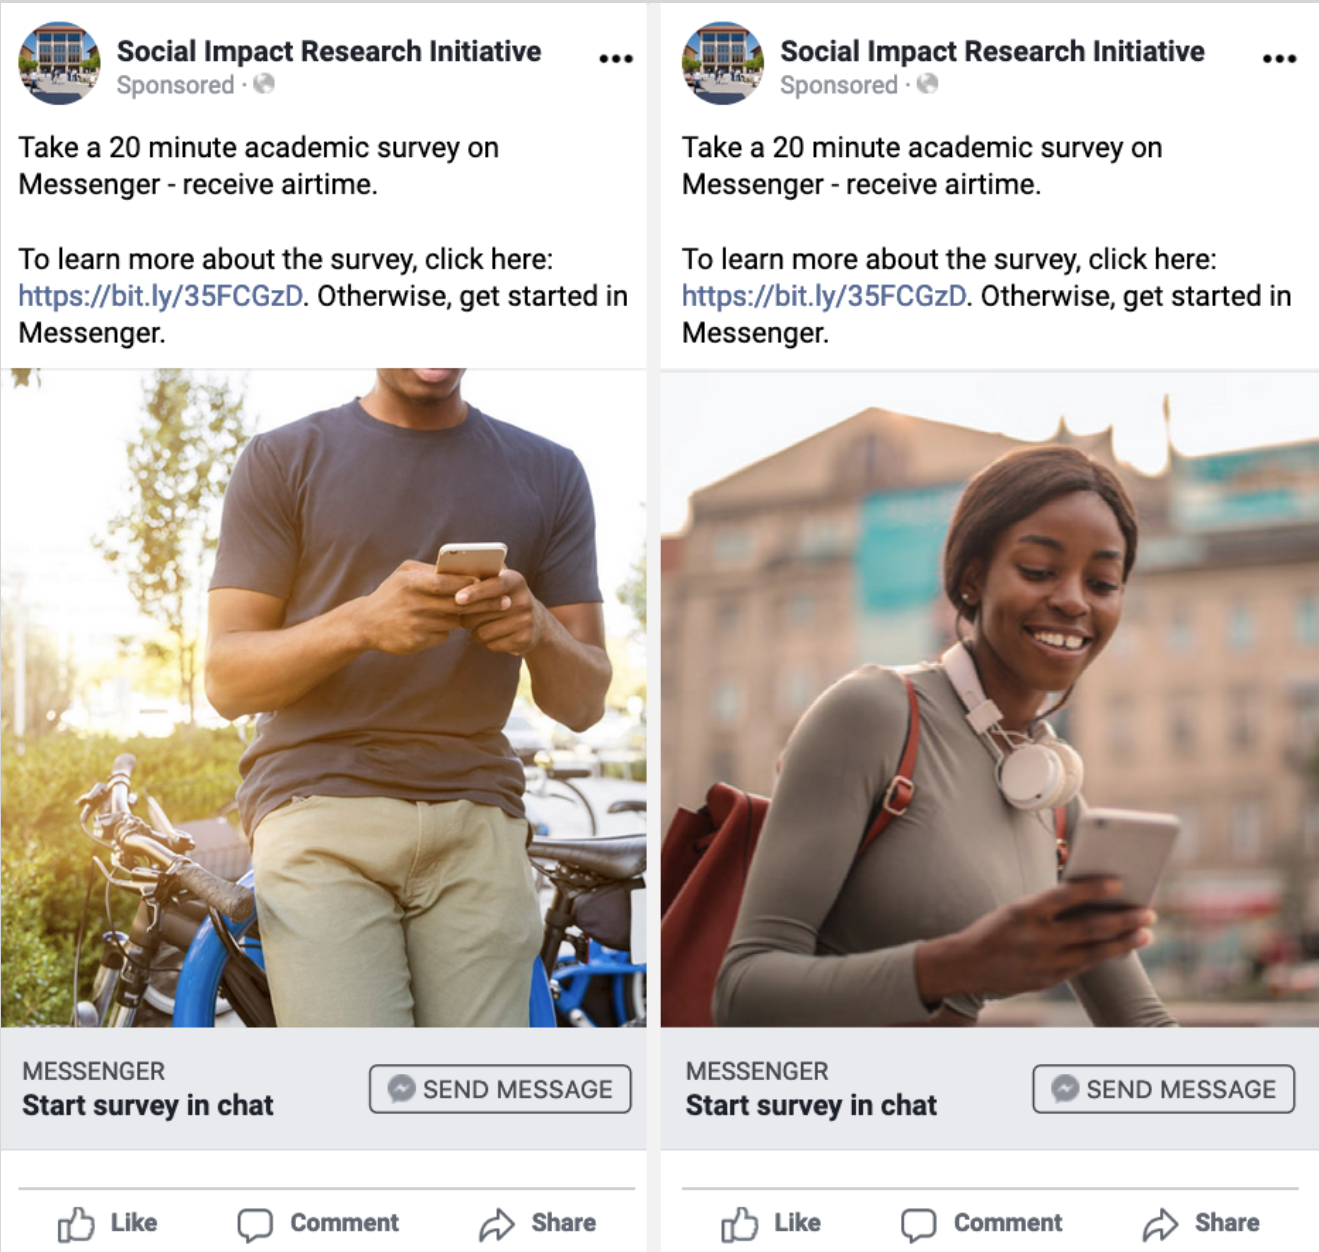
\includegraphics[width=.6\textwidth]{figures/advertisement_2020-10-26.png}
\end{figure}

After clicking on the ad, respondents are directed to the Chatbot (Figure \ref{fig:chatbot}) to take the survey.

\begin{figure}[htb]
\centering
\caption{Screenshot of Chatbot interface}
\label{fig:chatbot}
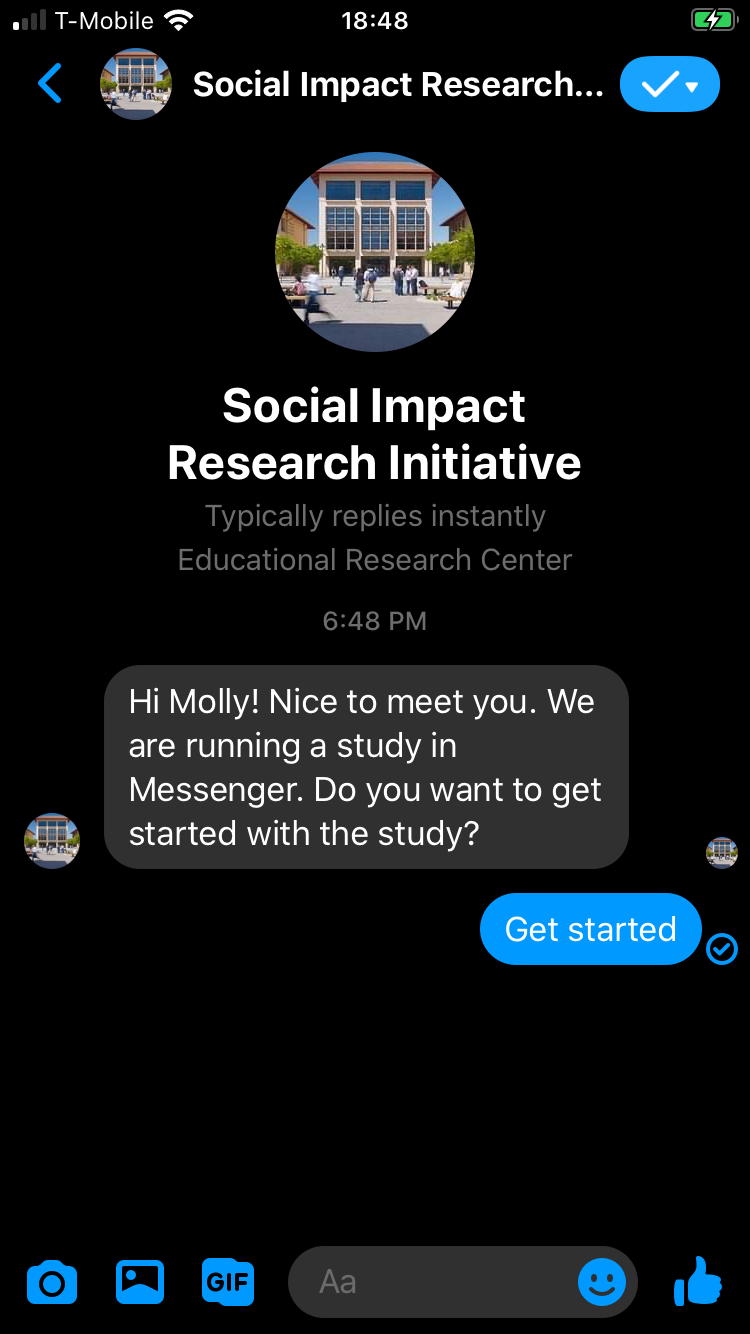
\includegraphics[width=.25\textwidth]{figures/chatbot_image.png}
\end{figure}

\section{Survey and data}\label{appendix:data}
\subsection{Covariates}\label{appendix:covariates}
\begin{table}[H]
\begin{adjustbox}{totalheight=.9\textheight-2\baselineskip, max width = \textwidth}
\begin{tabular}{p{0.3\linewidth}p{0.7\linewidth}p{0.25\linewidth}}
\textbf{Covariate}                   & \textbf{Response options} & \textbf{Coded as}                                     \\
\hline
Gender                                      & Male,   Female, Nonbinary, Other                           & 1 if male, 0 otherwise  \\
Age                                         & Integers                                                   & Continuous, {flag if greater than 120}              \\
Education &
  No   formal schooling, Informal schooling only, Some primary school, Primary   school completed, Some secondary school, Secondary school completed,   Post-secondary qualifications, Some university, University completed,   Post-graduate &
  1:10, flag if missing \\
Geography                                   & Urban, Rural                                 & 1 if urban, 0 otherwise \\
Religion                                    & Christian, Muslim, Other/None                           & Indicators              \\
Denomination (Christian)  & Pentecostal, Other  & Indicator (coded 1 if Pentecostal, 0 otherwise)\\
Religiosity   (freq. of attendance) &
  Never,   Less than once a month, One to three times per month, Once a week, More than   once a week but less than daily, Daily &
  1:6, flag if missing \\
%    Belief in God's control & 1. God will grant wealth and good health to all believers who have enough faith, 2. God doesn't always give wealth and good health even to believers who have deep faith & Indicator (coded 1 if answer is 1, 0 otherwise)\\
 Locus of control & 
% Some people feel they have completely free choice and control over their lives, while other people feel that what they do has no real effect on what happens to them. Please enter a number between 1 and 10, where 1 means "no choice at all" and 10 means "a great deal of choice" to indicate how much freedom of choice and control you feel you have over the way your life turns out 
[See survey instrument for full list] & 1:10, flag if missing\\
Index   of scientific views                 & [See   survey instrument for full questions and response options] & 0:2, flag if missing                     \\
Digital Literacy Index &  {[}Based on the first nine items of \cite{guessetal2020digital}'s  proposed measure, see  survey instrument for full questions and response options{]}& 0:24\\
Frequency of social media usage (x2)& {[}See   survey instrument for full questions and response options{]} & 0:3, flag if missing \\
Cognitive Reflection Test& {[}See   survey instrument for full questions and response options{]}& 0:3 (1 point for each correct response)\\
Index of household possessions%:   radio, tv, motorvehicle/motorcycle, computer/laptop, bank account, mobile   phone, bicycle 
&
  I/my household owns, Do not own [See survey instrument for items] &
  Continuous, sum of owned items, flag if all missing \\
Job   with cash income                      & Yes,   No                                                  & 1 if yes                \\
Number   of people in household             & Integers                                                   & Continuous, flag if missing              \\
Political affiliation & Governing party v. opposition & Indicator (coded 1 if associate with or voted for candidate from governing party, 0 otherwise)\\
Concern regarding COVID-19                  & Not at all worried, Somewhat worried,  Very   worried      & 1:3, flag if missing                     \\
%COVID-19 information & [Three True/False questions, see survey instrument for full questions] & 0:3 (1 point for each correct response)\\
Perceived government efficacy   on COVID-19 & Very   poorly, Somewhat poorly, Somewhat well, Very well   & 1:4, flag if missing \\
%Sources and frequency of news/media consumption &Never, Less than once a month, A few times a month, A few times a week, Once a day, Multiple times a day \ \  [See survey instrument for sources]  &  0:5 for \textit{each} of top three sources
{Strata of response to pre-test stimuli} & [Would share stimuli on timeline/via Messenger]& Indicators for strata (0:2) x (True + False = 2 types) $\times$ (timeline + Messenger = 2 channels) 
\end{tabular} 
\end{adjustbox}
\footnotesize
\textit{Note:} Regarding missingness flags, respondents must respond to chatbot questions to advance in the survey, but for contexts they may enter ``skip'' if they do not wish to answer a given question, with the exception of age, which we check is greater than 18. 
\caption{Covariates and response options}
\label{cov_long}
\end{table}

In all analyses, we include the pre-test response strata for true and false stimuli and indicators for individual stimuli.
For some continuous covariates that describe individual characteristics, such as education, we include an indicator flag if the respondent skipped the question; this is noted in the ``Coded as'' column. For others which require reflection or where there is a ``correct'' or ``best'' response, such as the Cognitive Reflection Test or the COVID-19 information measure, we we code the index as 0 if the respondent chose not to answer any of the questions. 

\subsection{Survey Instrument}\label{appendix:survey}%\todo{Check for update to public-facing survey instrument.}
The survey script is available at this link:\\
\url{https://docs.google.com/spreadsheets/d/1ZEi8xU-TOZCZIQnDqq4VYjG5cWjIaWNyoKvPCjLL3fg/edit#gid=366167997&range=A1}

\subsection{Stimuli}\label{appendix:stimuli}
All of the stimuli used in the experiment are available at this link:\\
\url{https://docs.google.com/spreadsheets/d/1ZEi8xU-TOZCZIQnDqq4VYjG5cWjIaWNyoKvPCjLL3fg/edit?usp=sharing}


\subsection{Treatments}\label{sec:treatments}
%\todo{Include mockups for headlines, full questions for respondent-level treatments, add deliberation stimuli and describe}
Additional details for the treatments described in Table~\ref{tab:treatments} are provided below. 


\subsubsection{Facebook Tips}\label{sec:fbtips}
The script for the Facebook tips respondent-level treatment is as follows:

As we're learning more about the Coronavirus, new information can spread quickly, and it's hard to know what information and sources to trust. Facebook has some tips for how to be smart about what information to trust. 

1. Be skeptical of headlines. False news stories often have catchy headlines in all caps with exclamation points. If shocking claims in the headline sound unbelievable, they probably are.©

2. Look closely at the link. A phony or look-alike link may be a warning sign of false news. Many false news sites mimic authentic news sources by making small changes to the link. You can go to the site to compare the link to established sources.

3. Investigate the source. Ensure that the story is written by a source that you trust with a reputation for accuracy. If the story comes from an unfamiliar organization, check their ``About'' section to learn more.

4. Watch for unusual formatting. Many false news sites have misspellings or awkward layouts. Read carefully if you see these signs.

5. Consider the photos. False news stories often contain manipulated images or videos. Sometimes the photo may be authentic, but taken out of context. You can search for the photo or image to verify where it came from.

6. Inspect the dates. False news stories may contain timelines that make no sense, or event dates that have been altered.

7. Check the evidence. Check the author's sources to confirm that they are accurate. Lack of evidence or reliance on unnamed experts may indicate a false news story.

8. Look at other reports. If no other news source is reporting the same story, it may indicate that the story is false. If the story is reported by multiple sources you trust, it's more likely to be true.

9. Is the story a joke? Sometimes false news stories can be hard to distinguish from humor or satire. Check whether the source is known for parody, and whether the story's details and tone suggest it may be just for fun.

10. Some stories are intentionally false. Think critically about the stories you read, and only share news that you know to be credible.



\subsubsection{AfricaCheck Tips}\label{sec:actips}
The script for the AfricaCheck tips respondent-level treatment is as follows:

As we're learning more about the Coronavirus, new information can spread quickly, and it's hard to know what information and sources to trust. AfricaCheck.org has some tips for how to be smart about what information to trust. 

1. Pause, particularly if the post, tweet or message makes you scared or angry. 

False or unverified information can spread quickly, especially if it makes you feel particular emotions.

2. Consider the source

When a friend or contact shares new information on Covid-19, it’s good to ask them: “How do you know that?” The answer can help you work out if they have first-hand knowledge of the information.

3. Try to find a trusted source

Check if fact-checking organisations have debunked the claim. For Covid-19, these are some good options:

First Draft\\
Africa Check\\
AFP Fact Check

%
%\subsubsection{Video Treatment}
%\label{sec:video}
%Respondents are shown one of the following videos, produced by BBC:
%
%\begin{itemize}
%\item \url{https://www.facebook.com/Vodcasts/videos/1322816708106278/}
%\item \url{https://www.facebook.com/BBCnewsafrica/videos/3104356182956064/}
%\item \url{https://www.facebook.com/BBCMediaActionNaija/videos/195932528440760/}
%\end{itemize}


\subsubsection{Accuracy and Deliberation Nudge Treatments}\label{sec:nudge}

For both the accuracy and deliberation nudge treatments, respondents will see the below placebo headline and asked the nudge question about it. For the accuracy nudge respondents are asked to think about whether the headline is true. The deliberation nudge asks respondents to think about why they would either choose to share or not share this headline.

\begin{figure}[htb]
\centering
    \begin{minipage}{0.45\textwidth}
        \centering
        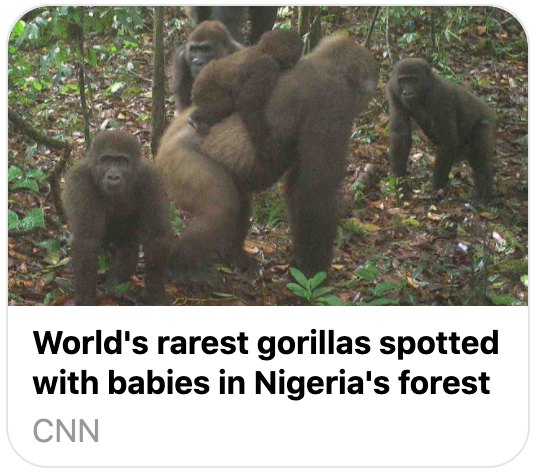
\includegraphics[width=\textwidth]{figures/placebo_ng.png} 
        \caption{Placebo headline for Nigerian respondents}
    \end{minipage}\hfill
    \begin{minipage}{0.45\textwidth}
        \centering
        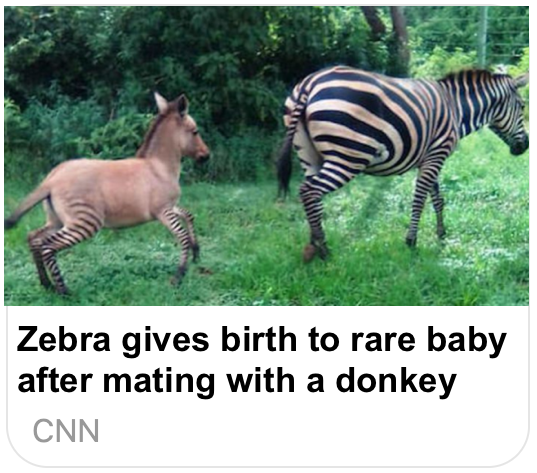
\includegraphics[width=\textwidth]{figures/placebo_ky.png} 
        \caption{Placebo headline for Kenyan respondents}
    \end{minipage}
\end{figure} 

\FloatBarrier


\subsubsection{Pledge Treatment}
\label{sec:pledge}
This treatment draws on the psychological evidence around commitment and consistency \citep{cialdini1987influence,costa2018walking}. Knowing that people, as much as possible, want to appear consistent with their prior words and actions, we want to see whether we can first get them to commit to an ``easy ask'' and then lead them down a path towards a public (or private) pledge.


\begin{enumerate}

\item Do you want to keep your family, friends and community safe from COVID-19? (Yes!, No)
\\\textit{If "No" $\rightarrow$ end}

\item Did you know that false information about ways to prevent or cure COVID-19 threaten the health and well-being of everyone around us?  (Yes, No)

\item Are you committed to keeping your family, friends, and community safe from COVID-19 misinformation? (Yes!, No)
\\\textit{If "No" $\rightarrow$ end}

\item Great! Take our pledge by posting this image [here/to your timeline] now.
\\NOTE: \textit{Respondents are randomized to either be asked to take the pledge privately, within the chatbot, or to post the pledge publicly to their timeline.}

%\item IF 1=YES: Are you committed to stopping the spread of harmful/dangerous false information about COVID-19 online? (yes, no)
%\item IF 1=NO: Why not? [open response]
%
%\textit{Respondents in pledge treatment will be randomized (equal and static assignment probability) to either see the public or private pledge below}
%
%\item \textbf{public pledge:}\\
%IF 2=YES:  Great! Please take our pledge by posting this pledge to your timeline now. \\ IF 2=NO: Why not? [open response]
%
%\item \textbf{private pledge:}\\
%IF 2=YES:  Great! Please take our pledge now by posting it here. \\
%IF 2=NO: Why not? [open response]

\begin{figure}[htb]
\centering
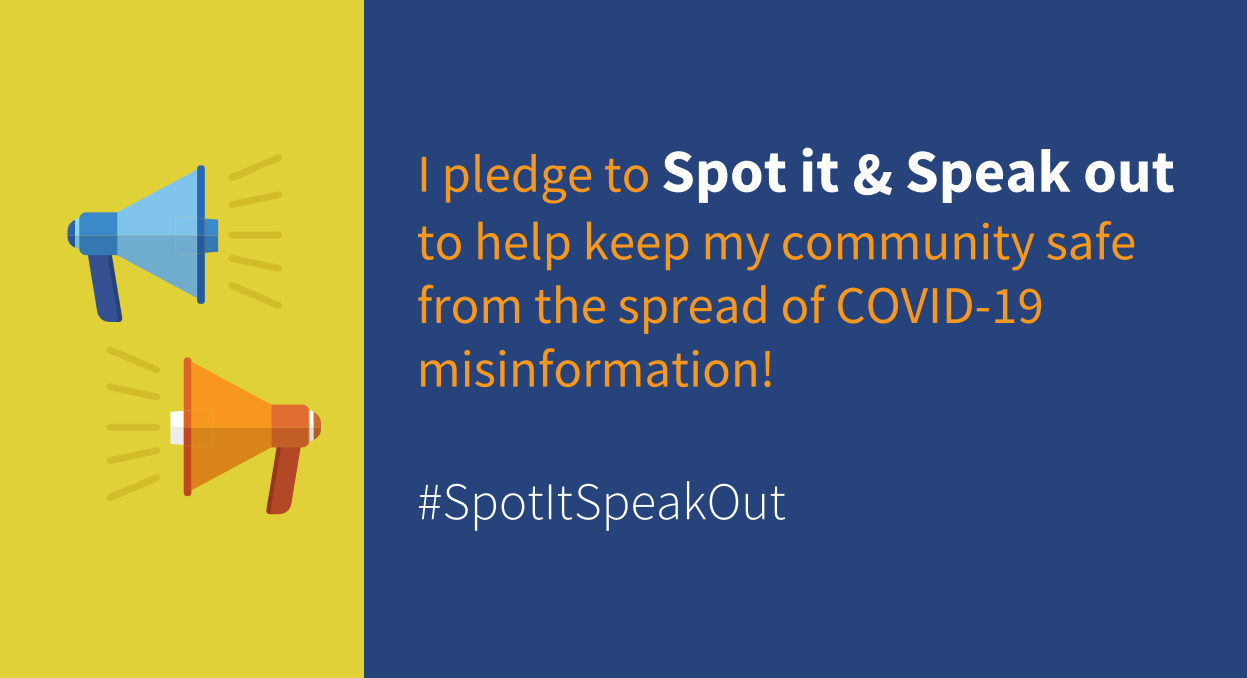
\includegraphics[width=.5\textwidth]{figures/pledge_image.png}
\caption{Pledge infographic respondents are asked to post \textit{privately} to the chatbot or \textit{publicly} to their timeline. During the pilot we will randomize and test elements of this pledge by varying whether ``community'' or ``family and friends'' is the more effective reference group.}
\end{figure}
\end{enumerate}


\subsubsection{Headline Level Treatments}
%Samples of the three headline-level treatments appear below:

\begin{figure}[htb]
\centering
    \caption{Headline treatments}
    \label{headline_treatments}
    \begin{minipage}{0.4\textwidth}
        \centering
        
\includegraphics[width=\textwidth]{figures/treat_relatedarticles.png} 
        \caption*{Related Articles}
    \end{minipage}\hfill
    \begin{minipage}{0.4\textwidth}
        \centering
        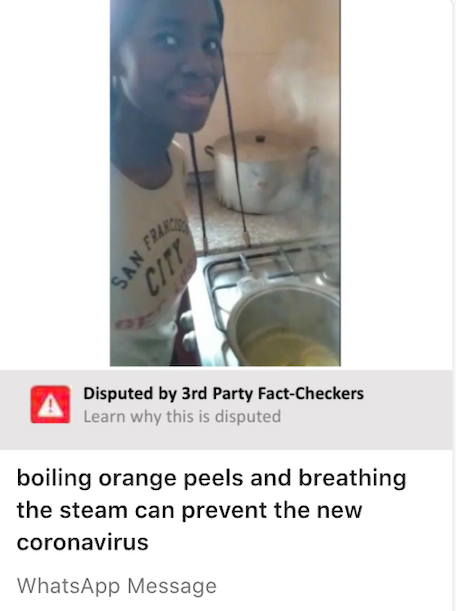
\includegraphics[width=\textwidth]{figures/treat_factcheck.png} 
        \caption*{Factcheck}
    \end{minipage}
    \vspace{1in}
    \begin{minipage}{0.4\textwidth}
        \centering
        
\includegraphics[width=\textwidth]{figures/treat_moreinfo.png} 
        \caption*{More information}
    \end{minipage}\hfill
     \begin{minipage}{0.45\textwidth}
        \centering
        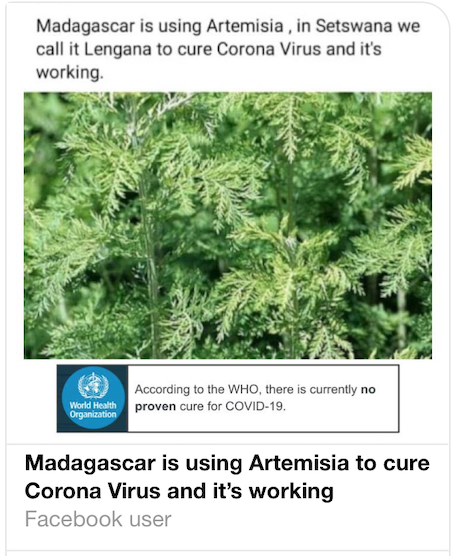
\includegraphics[width=\textwidth]{figures/treat_realinfo.png} 
        \caption*{Real information}
    \end{minipage}
\end{figure}

\FloatBarrier
\section{Batch-wise balanced linear Thompson sampling}\label{appendix:agent}

A note on notation: while $X_i$ represents the covariates observed for individual $i$, the covariate vector $X_{[W]i}$ is in the appropriate format for the relevant counterfactual treatment indicators and interactions--i.e., for each observation, we can generate this vector for every hypothetical treatment. For ease of notation, we let $\X$ be the covariate matrix for the covariates augmented with thei respective realized treatments. 


\begin{algorithm} \footnotesize
    \caption{Batch-wise balanced linear Thompson sampling}
    \label{algg:bblts}
    \begin{algorithmic}[1] % The number tells where the line numbering should start
    	\State$\Xi \leftarrow$ empty matrix; $\X \leftarrow$ empty matrix; $\y \leftarrow$ empty vector. %for $w \in \ww$. 
	\Comment{Initialize weight matrix, treatment-augmented covariate matrix, and reward vector.  
	}
    	\For{$i = 1, \dots, N$}
		\If{$i \in \mathcal{I}_1$}
			 \State $e_{w} \leftarrow \frac{1 }{|\ww| } \ \ \forall w \in \ww $ \Comment{In first batch, assign treatment uniformly at random.}
		\ElsIf{$i \in \mathcal{I}_b$ for $b = 2, \dots, B$}
			\If{$i$ is the first observation in $\mathcal{I}_b$} \Comment{Update estimates of coefficient vector and variance matrix, using ridge regression with determined penalization.}
%				\For{$w\in \ww$}
%					\State $B_w \leftarrow X^\top_w \Xi_w X_w + \lambda^{CV} \mathbf{I}$ 
%					\State $\hat\theta_{w} \leftarrow B_w^{-1} X_w^\top \Xi_w r_w$
%					\State $\hat\V[\hat\theta_{w}] \leftarrow B_w^{-1} \left(\left( r_w - X_w^\top\hat\theta_{w} \right)^\top \Xi_w \left( r_w - X_w^\top\hat\theta_{w} \right)\right)$
%				\EndFor
				\State $B \leftarrow \X^\top \Xi \X + \lambda^{CV} \mathbf{I}$  
				\State $\hat\theta \leftarrow B^{-1} \X^\top \Xi y$
				\State $\hat\V[\hat\theta] \leftarrow B^{-1} \left(\left( \y - \X^\top\hat\theta \right)^\top \Xi \left( \y - \X^\top\hat\theta \right)\right)$
			\EndIf
			\For{$m = 1, \dots, M$}
				\State Sample $\tilde \theta^{(m)}  \sim \mathcal{N}\left(\hat\theta, \hat\V[\hat\theta] \right)$
			 \EndFor
				\State $q_w \leftarrow \frac{1}{M} \sum_{m=1}^M 1\left\{ w = \underset{w}{\argmax} \{ x_{[1]i}^\top \tilde \theta ^{(m)}, \dots, x_{[|\ww|]i}^\top\tilde \theta^{(m)} \}  \right\}$ \Comment{ Compute TS probabilities based on observed context.}
     			\State $\tilde{q}_w =\max\left\{q_w, p\right\}\ \ \forall w \in \ww$ \Comment{Impose probability floors,}
			\State $u_{\textrm{total}} = \sum_w \tilde{q}_w - 1$ \Comment{ and rescale. }
			\State $u_{w} = \tilde{q}_w - p \ \ \forall w \in \ww$
			\State $ c = u_{\textrm{total}} / \left( \sum_w u_{w} \right)$
			\State $e_w = \tilde{q}_w -c*u_{w} \ \ \forall w \in \ww$
%	def apply_floor(a, amin):
%    new = np.maximum(a, amin)
%    total_slack = np.sum(new) - 1
%    individual_slack = new - amin
%    c = total_slack / np.sum(individual_slack)
%    return new - c * individual_slack			
% 			\State ${e}_w = \frac{ \tilde{q}_w}{\sum\limits_{w }\tilde{q}_w }\ \ \forall w \in \ww$ \Comment{ and rescale. }
%			\State $e_{w_C}(X_{[W]i})  = 0.2 + 0.8\hat{q}_{w_C}(X_{[W]i}) $ \Comment{Augment the control with a fixed probability. }
%                         \State $e_{w}(X_{[W]i})  = 0.8\hat{q}_w(X_{[W]i}) \ \ \forall w \in \ww \setminus \{w_C\}$ \Comment{Ensure probabilities sum to 1.}  
		\EndIf
		\State Assign $w_i \sim \textrm{Multinom}( e_{1}, \dots,  e_{|\ww|} )$ \Comment{Assign treatment.}
		\State $\xi_i \leftarrow \frac{ 1 }{e_{w_i}}$ \Comment{Record inverse probability weights based on realized assignment.}
		\State $\Xi \leftarrow \diag \left(\Xi, \xi_i\right)$ \Comment{Augment weight matrix.}
		\State $\X \leftarrow [\X:x_{[w_i]i}^\top]$ \Comment{Augment covariate matrix.}
		\State $\y \leftarrow  [\y: y_i]$ \Comment{Augment reward vector.}
	\EndFor
    \end{algorithmic}
\end{algorithm}

\clearpage


\section{Estimation Considerations}

%\subsection{Inverse probability weighting} \label{appendix:stabilized}

%In ex post evaluation, we use the stabilized version of these weights, normalizing weights to sum to one on the empirical data. This may improve RMSE of the estimator \citep{cole2008constructing}. 
%\begin{align}
%\left.
%\xi^{SIPW}_w(X_i) = \frac{ 1 }{e_{w}(X_i)}
%\middle/ 
%{ \sum_{j = 1}^N \frac{1\{W_{j} = w\}}{e_{w}(X_j)} } \label{eq:SIPW} \numberthis
%\right.
%\end{align}
%
%For batched adaptively collected data, we sum over all observations in the same batch. %todo{Could formalize this.}
%
%\begin{align}
%\left.
%\xi^{SIPW}_{b,w}(X_i) = \frac{ 1 }{e_{w}^{\pi^{(b)}}(X_i)}   
%\middle/ 
%{ \sum_{j = 1}^\top \frac{1\{W_{j} = w\}}{e_{w}^{\pi^{(B_j)}}(X_i)} } \label{eq:SIPWb} \numberthis
%\right.
%\end{align}


%\subsection{Random best fixed policies}\label{appendix:bestfixed}
%We may be interested in learning and evaluating the best fixed policy. However, if we learn which fixed policy is best by taking the fixed policy with the highest mean, we get a biased estimate of the best fixed policy. To see this, consider:
%\begin{align*}
%\E[\max(X_1, \dots, X_N)] \ge \max(\E[X_1],\dots, \E[X_N]). 
%\end{align*}
%
%To address this concern, we consider instead a \textit{random} best fixed policy. We use only IPW scores, \textit{not} the doubly robust scores, to avoid the additional dependence in estimates produced by conditional means model. 
%\begin{enumerate}
%\item For each observation $i>1$ in the experiment, we calculate the value of fixed policies as the average of scores up to time $i-1$. 
%\begin{align*}
%\hat{V}_{i-1}({\pi}_{w})  &:= \frac{1}{i-1 } \sum_{j = 1 }^{i-1} \hat{\Gamma}_{j,w} \quad \text{for fixed policies $w$}
%\end{align*}
%\item The ``best'' fixed policy in period $i$ is the treatment with the highest estimate:
%\begin{align*}
%w_i^* =  \argmax_w \ \hat{V}_{i-1}({\pi}_{w})
%\end{align*}
%\item The score for the random best fixed policy in time $i$ is then the score in that period for the selected arm, $\hat{\Gamma}_{i, w^*}$ 
% \item To evaluate the policies, we again take the average scores. The evaluation set $\mathcal{I}^*$ will be the entire data set for data collected under the procedures for the random agent as described above in Section~\ref{randomlearning}, and up through batch $B-1$ for data collected under the procedures for the adaptive agent--excluding the first observation. 
%    \begin{align*}
%          \hat{V}(\hat{\pi}_{w^*})  &:= \frac{1}{\big{\lvert} \mathcal{I}^* \big{\rvert}} \sum_{i \in \mathcal{I}^* } 
%          \hat{\Gamma}_{i, w_i^*} 
%  \end{align*}
%\end{enumerate}

\subsection{Policy evaluation on randomly collected data}\label{randomlearning}

%\subsection{Random forest estimation}\label{appendix:grf}
Data is collected by assigning treatment uniformly at random. This means that we do not need to account for historical dependencies in the data when estimating nuisance components. We still split data to learn and evaluate policies on separate splits of the data; for comparison to the adaptively collected data, we also imagine ``batches'' of the same size as those collected in an adaptive experiment, but in practice these are only meaningful for determining the size of the last batch held out for evaluation. 
\begin{enumerate}
  \item \textbf{Compute doubly robust scores.} For weights  $\hat\xi_w(X_i)$, use assigned probabilities $1/|\ww|$. To estimate conditional means $\hat \mu_w(X_i)$, using \textit{all} data in $b$ in $b = 1, \dots, B-1$, for each treatment $w$:
\begin{enumerate}
\item Fit a random forest estimator on the observations assigned $w$. 
\item For observations assigned $w$, calculate $\hat\mu_w(X_i)$ using out-of-bag predictions. 
\item For observation \textit{not} assigned $w$, calculate $\hat\mu_w(X_i)$ using regression forest predictions from the fitted model in step a. 
\end{enumerate}
 Compute doubly robust scores $\hat{\Gamma}_{i,w}$ plugging the estimated nuisance components into (\ref{eq:DR}). 
%  \item Compute doubly robust scores $\hat{\Gamma}_{i,w}$ substituting the estimated nuisance components into (\ref{eq:DR}). 
%%  \item Separating the data into $k$ folds, fit optimal depth\textcolor{black}{-two} policy tree leaving out the $k$\textsuperscript{th} fold:
%%    \begin{align*}
%%      \hat{\pi}_{opt}^{-k} = \arg\max_{\pi \in \Pi}
%%       \sum_{i \in \mathcal{I}_{-k}}
%%      \langle \pi(X_{i}), \hat{\Gamma}_{i, \cdot} \rangle \\
%%       \text{where } \Pi \text{ is the class of depth-\textcolor{black}{two} policy trees.}
%%    \end{align*}
%%% Point-wise optimal random forest  
%%  \item Fit a point-wise optimal contextual policy $\hat{\pi}_{opt}$ by taking the maximum of predicted values at each point
%%    \begin{equation*}
%%\hat{\pi}_{x_i}  =     \argmax_{w} \hat{\mu}_{w}(x_i) 
%%    \end{equation*}
%  \item To evaluate the policies, take the average scores :
%    \begin{align*}
%          \hat{V}({\pi}_{w})  &:= \frac{1}{N} \sum_{i}^N \hat{\Gamma}_{i,w} \\
%      \hat{V}(\hat{\pi}_{opt})  
%      %% Point-wise optimal random forest  
%      % &:= \frac{1}{N} \sum_{i}^N \hat{\Gamma}_{i, \hat{\pi}_{X_i}} 
%					 &:= \frac{1}{K} \sum_{k}^K  \frac{1}{|\mathcal{I}_{-k}|} \sum_{i \in \mathcal{I}_{-k} }
%          \langle \hat{\pi}_{opt}^{-k}(X_{t}), \hat{\Gamma}_{i, \cdot} \rangle
%          \end{align*}
%%   \item To learn and evaluate the best fixed policy on a dataset, we cannot simply take the treatment condition with the highest estimated value, as this will give us positive bias in expectation. To account for this, we use the approach described in Appendix~\ref{appendix:bestfixed}. 
\end{enumerate}

Complete steps 2 and 3 as described in Section~\ref{adaptivelearning}. 



\section{Pre-experimental simulation DGP}\label{appendix:dgp}

Objective for DGPs:
\begin{itemize}
    \item Create multiple clusters, where distributions of covariates are different across clusters
    \item Each cluster has a different arm that produces highest reward
    \item Generate ``lumpy'' reward functions that cannot be straightforwardly recovered by a linear model
    \item Allow levers to move:
    \begin{itemize}
        \item number of covariates used to define clusters
        \item relative size of clusters
        \item \textit{Heterogeneity delta} (relative value of best contextual/best fixed policy)
    \end{itemize} 
\end{itemize}

Requirements for DGPs:
\begin{itemize}
    \item The difference between the best contextual policy \& the control is fixed across DGPs
    \begin{itemize}
        \item[$\Rightarrow$] Differences in power curves between DGPs are based on ability of agent to learn the DGP, not differences in effect sizes
    \end{itemize}
    \item The best fixed arm is always the same arm across DGPs (In the simulations, arm 0 is chosen as the best arm for the largest cluster. It is also chosen as the 2nd best arm for the other two clusters to ensure it is the best-fixed policy.)
\end{itemize}


\textbf{Generate Baseline Dataset ($N = 10,000, p = 15$)}
\begin{itemize}
    \item Parameter \begin{itemize}
%        \item Number of useful covariates $p' \in \{3, 5, 10\}$ (i.e., covariates used to determine cluster membership)
        \item Number of useful covariates $p' \in \{3, 5\}$ (i.e., covariates used to determine cluster membership)
        \item Largest cluster size ratio $c \in \{0.4, 0.6, 0.8\}$
        \item Heterogeneity delta $h \in \{0.02, 0.14, 0.2\}$
    \end{itemize}
    \item Generate large covariate matrix $\X'$ using correlated multivariate normal distribution, covariance matrix generated from $\frac{Beta(2,2) - 0.5}{2}$, where the dimension is $N \times p'$. We then add $p - p'$ columns of noise generated using a standard normal distribution to form the full covariate matrix $\X$.
    \item Use iterative KNN to group covariates observed into $k = 3$ clusters with cluster size [$N*c, \frac{N * (1-c)}{2}, \frac{N * (1-c)}{2}$], where $c$ = largest cluster size ratio
\end{itemize}

\textbf{Reward Generation}
\begin{itemize}
   \item We generate rewards only relying on the first column of the covariate matrix $\X$, denoted as $X_1$
    \item Generate reward for best arm $w_{best}$ for each cluster $c_i,  \ i = 1, \dots, 3$, \[R_{w_{best, i}, c_i} = 0.6 - X_{1, c_i}\]
    \item Reward for 2nd best arm, $w_{best_2}$ for each cluster $c_i,  i = 1, \dots, 3$, where we vary $\mu$ to search for the level of desired heterogeneity delta $h$
    $$R_{w_{best_2, i}, c_i} = R_{w_{best, i}, c_i} + \epsilon_R $$ where $\epsilon_R \sim \mathcal{N}(\mu, 0.01), -0.6 \le \mu \le 0$. 
    \item Rewards for the rest of the arms
    $$R_{w, c_i} = -X_{1, c_i} \mbox{ for }  w \not\in \{w_{best, i}, w_{best_2, i}\}, i = 1, \dots, 3.$$
    \item We vary $\mu$ to search for the level of desired heterogeneity delta $h$.
        \item[$\Rightarrow$] Cluster membership defines groups over which there is heterogeneity, and we also have a separate lever to move the magnitude of the heterogeneity in treatment effects, which comes from how we vary the noise reward $\epsilon_R$ to add to the 2nd best arm. 
\end{itemize}

\section{Variance calculation}

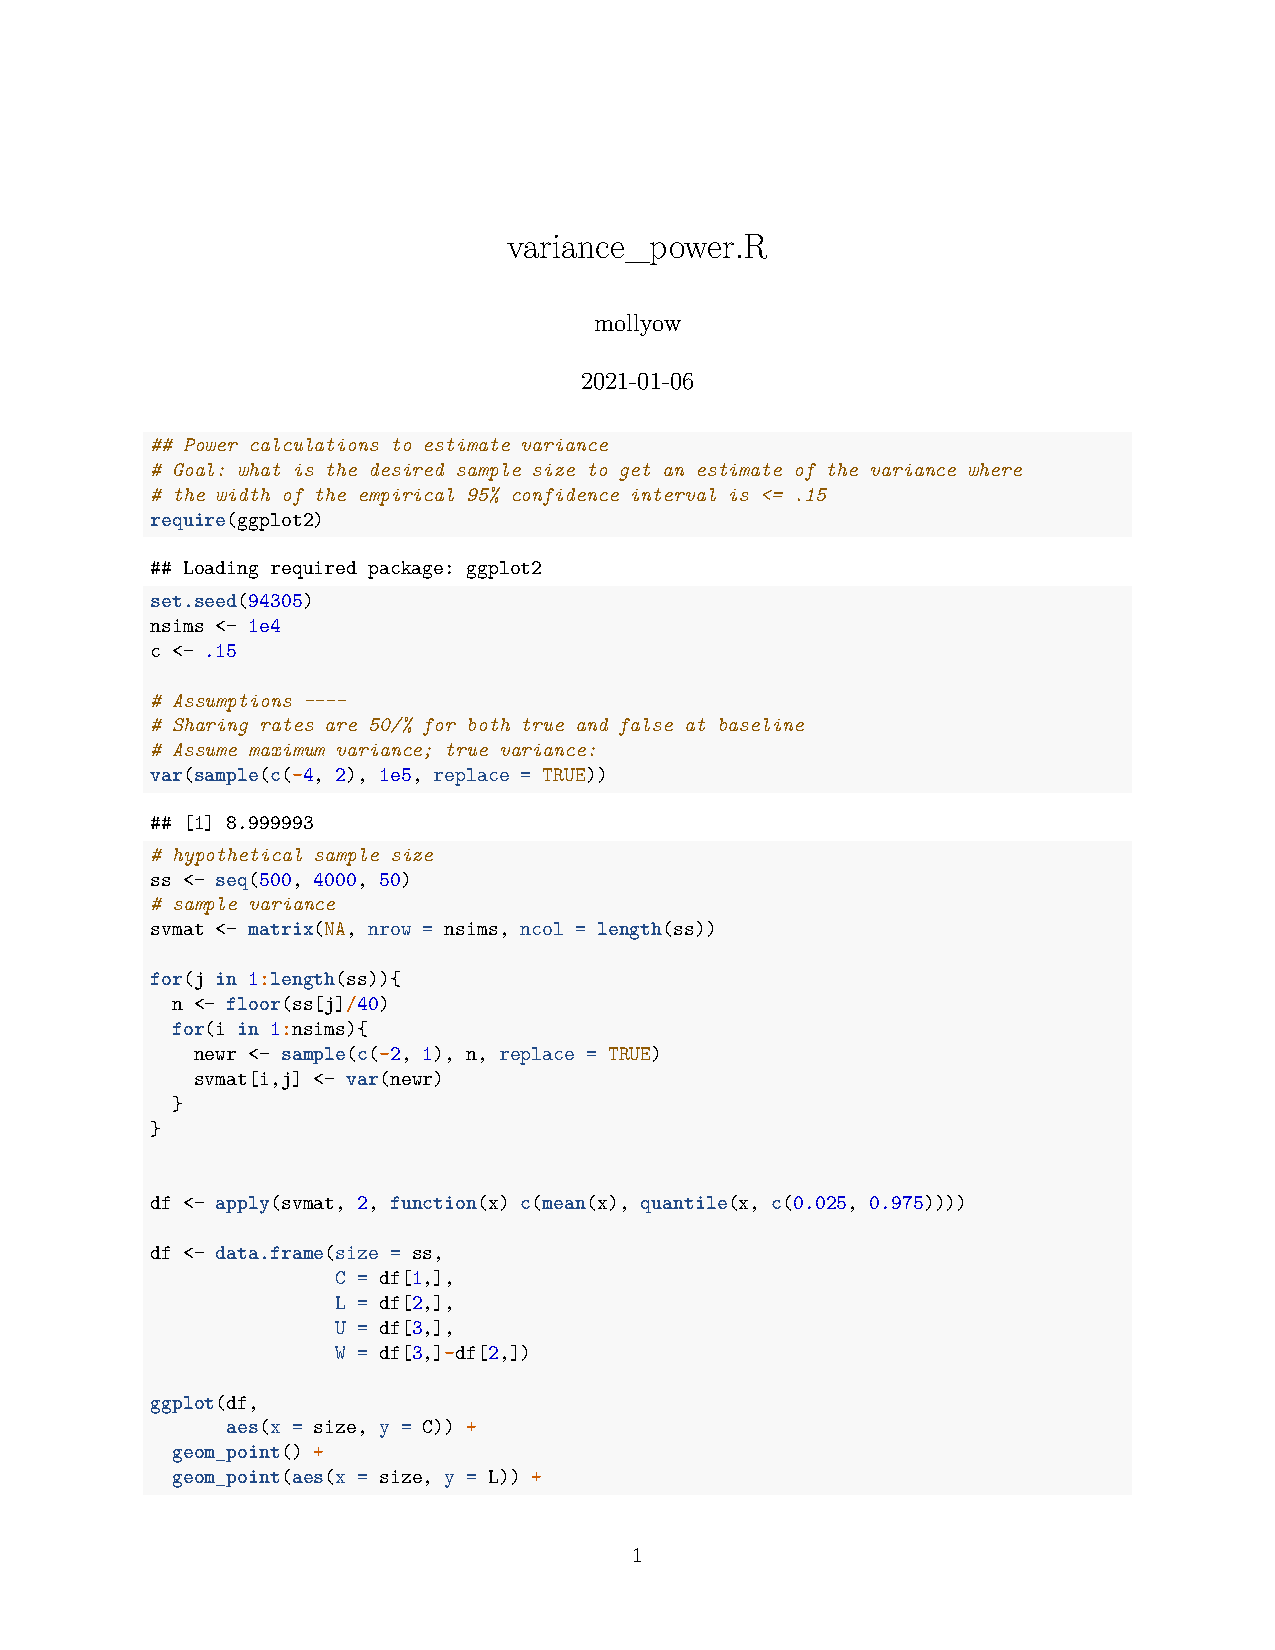
\includepdf[pages=-,pagecommand={},width=\textwidth]{variance_power.pdf}

\end{document}
